\chapter{Marco Práctico}

El presente capítulo describe la implementación, validación y 
resultados del simulador neuromórfico desarrollado. Se presenta 
en primer lugar la arquitectura general del sistema y las 
herramientas empleadas durante el desarrollo. Posteriormente se 
detalla la metodología seguida por etapas, desde el modelado del 
dispositivo memristivo hasta su integración en un agente de 
control autónomo. Finalmente se exponen los resultados 
experimentales obtenidos y se cierra con un análisis de costos 
asociado al desarrollo del sistema y su replicabilidad.

% =====================================================
\section{Esquema general del proyecto}
% =====================================================

La solución desarrollada se estructuró como un ecosistema 
computacional compuesto por dos subsistemas acoplados. El 
primero, denominado \textit{Neuromorphic Lab}, constituye el 
motor físico encargado de modelar dispositivos memristivos, 
neuronas tipo Leaky Integrate-and-Fire y arreglos crossbar con 
efectos no ideales. El segundo, denominado \textit{Robot Sim}, 
implementa un agente de control autónomo que utiliza el arreglo 
crossbar como sustrato físico de su política.

La Figura~\ref{fig:esquema_general} presenta la organización 
general de ambos subsistemas y su relación unidireccional: el 
simulador robótico consume los modelos físicos del laboratorio 
a través de una capa de abstracción (\textit{lab\_bridge}), 
pero el laboratorio no conoce la existencia del agente.

\begin{figure}[H]
\centering
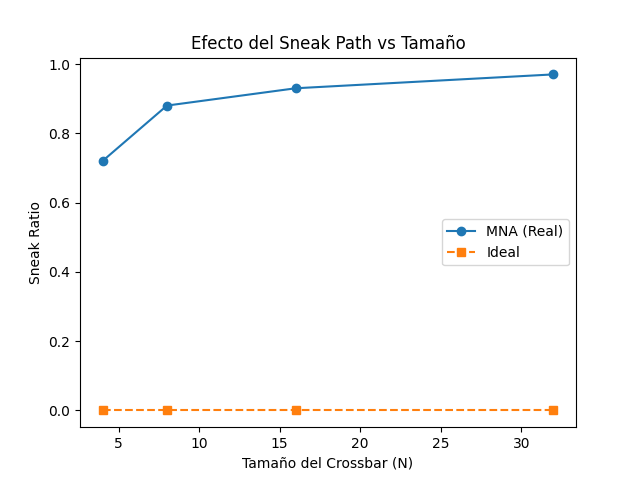
\includegraphics[width=\textwidth]{figuras/esquema_general.png}
\caption{Arquitectura general del ecosistema. El laboratorio 
(\textit{arriba}) provee los modelos físicos; el simulador 
robótico (\textit{abajo}) los integra en un agente de control.}
\label{fig:esquema_general}
\end{figure}

El flujo de información del agente sigue la secuencia 
\textit{sensores} $\rightarrow$ \textit{codificador} 
$\rightarrow$ \textit{crossbar} $\rightarrow$ \textit{decodificador} 
$\rightarrow$ \textit{actuadores}, con el aprendizaje aplicado al 
final de cada episodio mediante una regla de plasticidad 
modulada por recompensa. El detalle de cada componente se 
desarrolla en la Sección~\ref{sec:desarrollo}.

% =====================================================
\section{Herramientas}
% =====================================================

\subsection{Hardware}
% (vacío)

\subsection{Software}
% (vacío)

% =====================================================
\section{Desarrollo}
\label{sec:desarrollo}
% =====================================================

El desarrollo del simulador siguió una estrategia bottom-up: 
primero se validó el dispositivo individual, luego la neurona, 
después la plasticidad, y finalmente la integración en 
arquitecturas matriciales y en un agente de control. Cada etapa 
se verificó cuantitativamente contra resultados publicados antes 
de avanzar a la siguiente.

\subsection{Etapa 1 -- Modelado del dispositivo memristivo}

Se implementaron tres modelos físicos de memristor: el modelo 
analítico de Strukov et al. (2008) para dispositivos de dióxido 
de titanio, el modelo asimétrico de Yakopcic y Prezioso para 
dispositivos de capa fina Al$_2$O$_3$/TiO$_{2-x}$, y un modelo 
de memristor volátil basado en HfO$_2$ con relajación espontánea.

El modelo de Strukov describe la evolución de una variable 
interna $x(t) \in [0,1]$ que representa la frontera entre las 
regiones dopada y no dopada del dispositivo. La resistencia 
instantánea se calcula como combinación lineal convexa de los 
límites resistivos $R_{ON}$ y $R_{OFF}$. El modelo de Prezioso 
incorpora histéresis asimétrica SET/RESET mediante funciones 
hiperbólicas y umbrales de conmutación dependientes de 
polaridad. El modelo volátil añade un término de decaimiento 
exponencial hacia el estado basal, reproduciendo la dinámica 
de disolución del filamento conductivo.

La Figura~\ref{fig:validacion_memristor} compara las curvas 
$I$--$V$ obtenidas por el simulador contra los datos 
digitalizados de Strukov et al. (2008) y Prezioso et al. 
(2014). La concordancia alcanza un coeficiente de determinación 
$R^2 > 0.96$ en todas las ramas.

\begin{figure}[H]
\centering
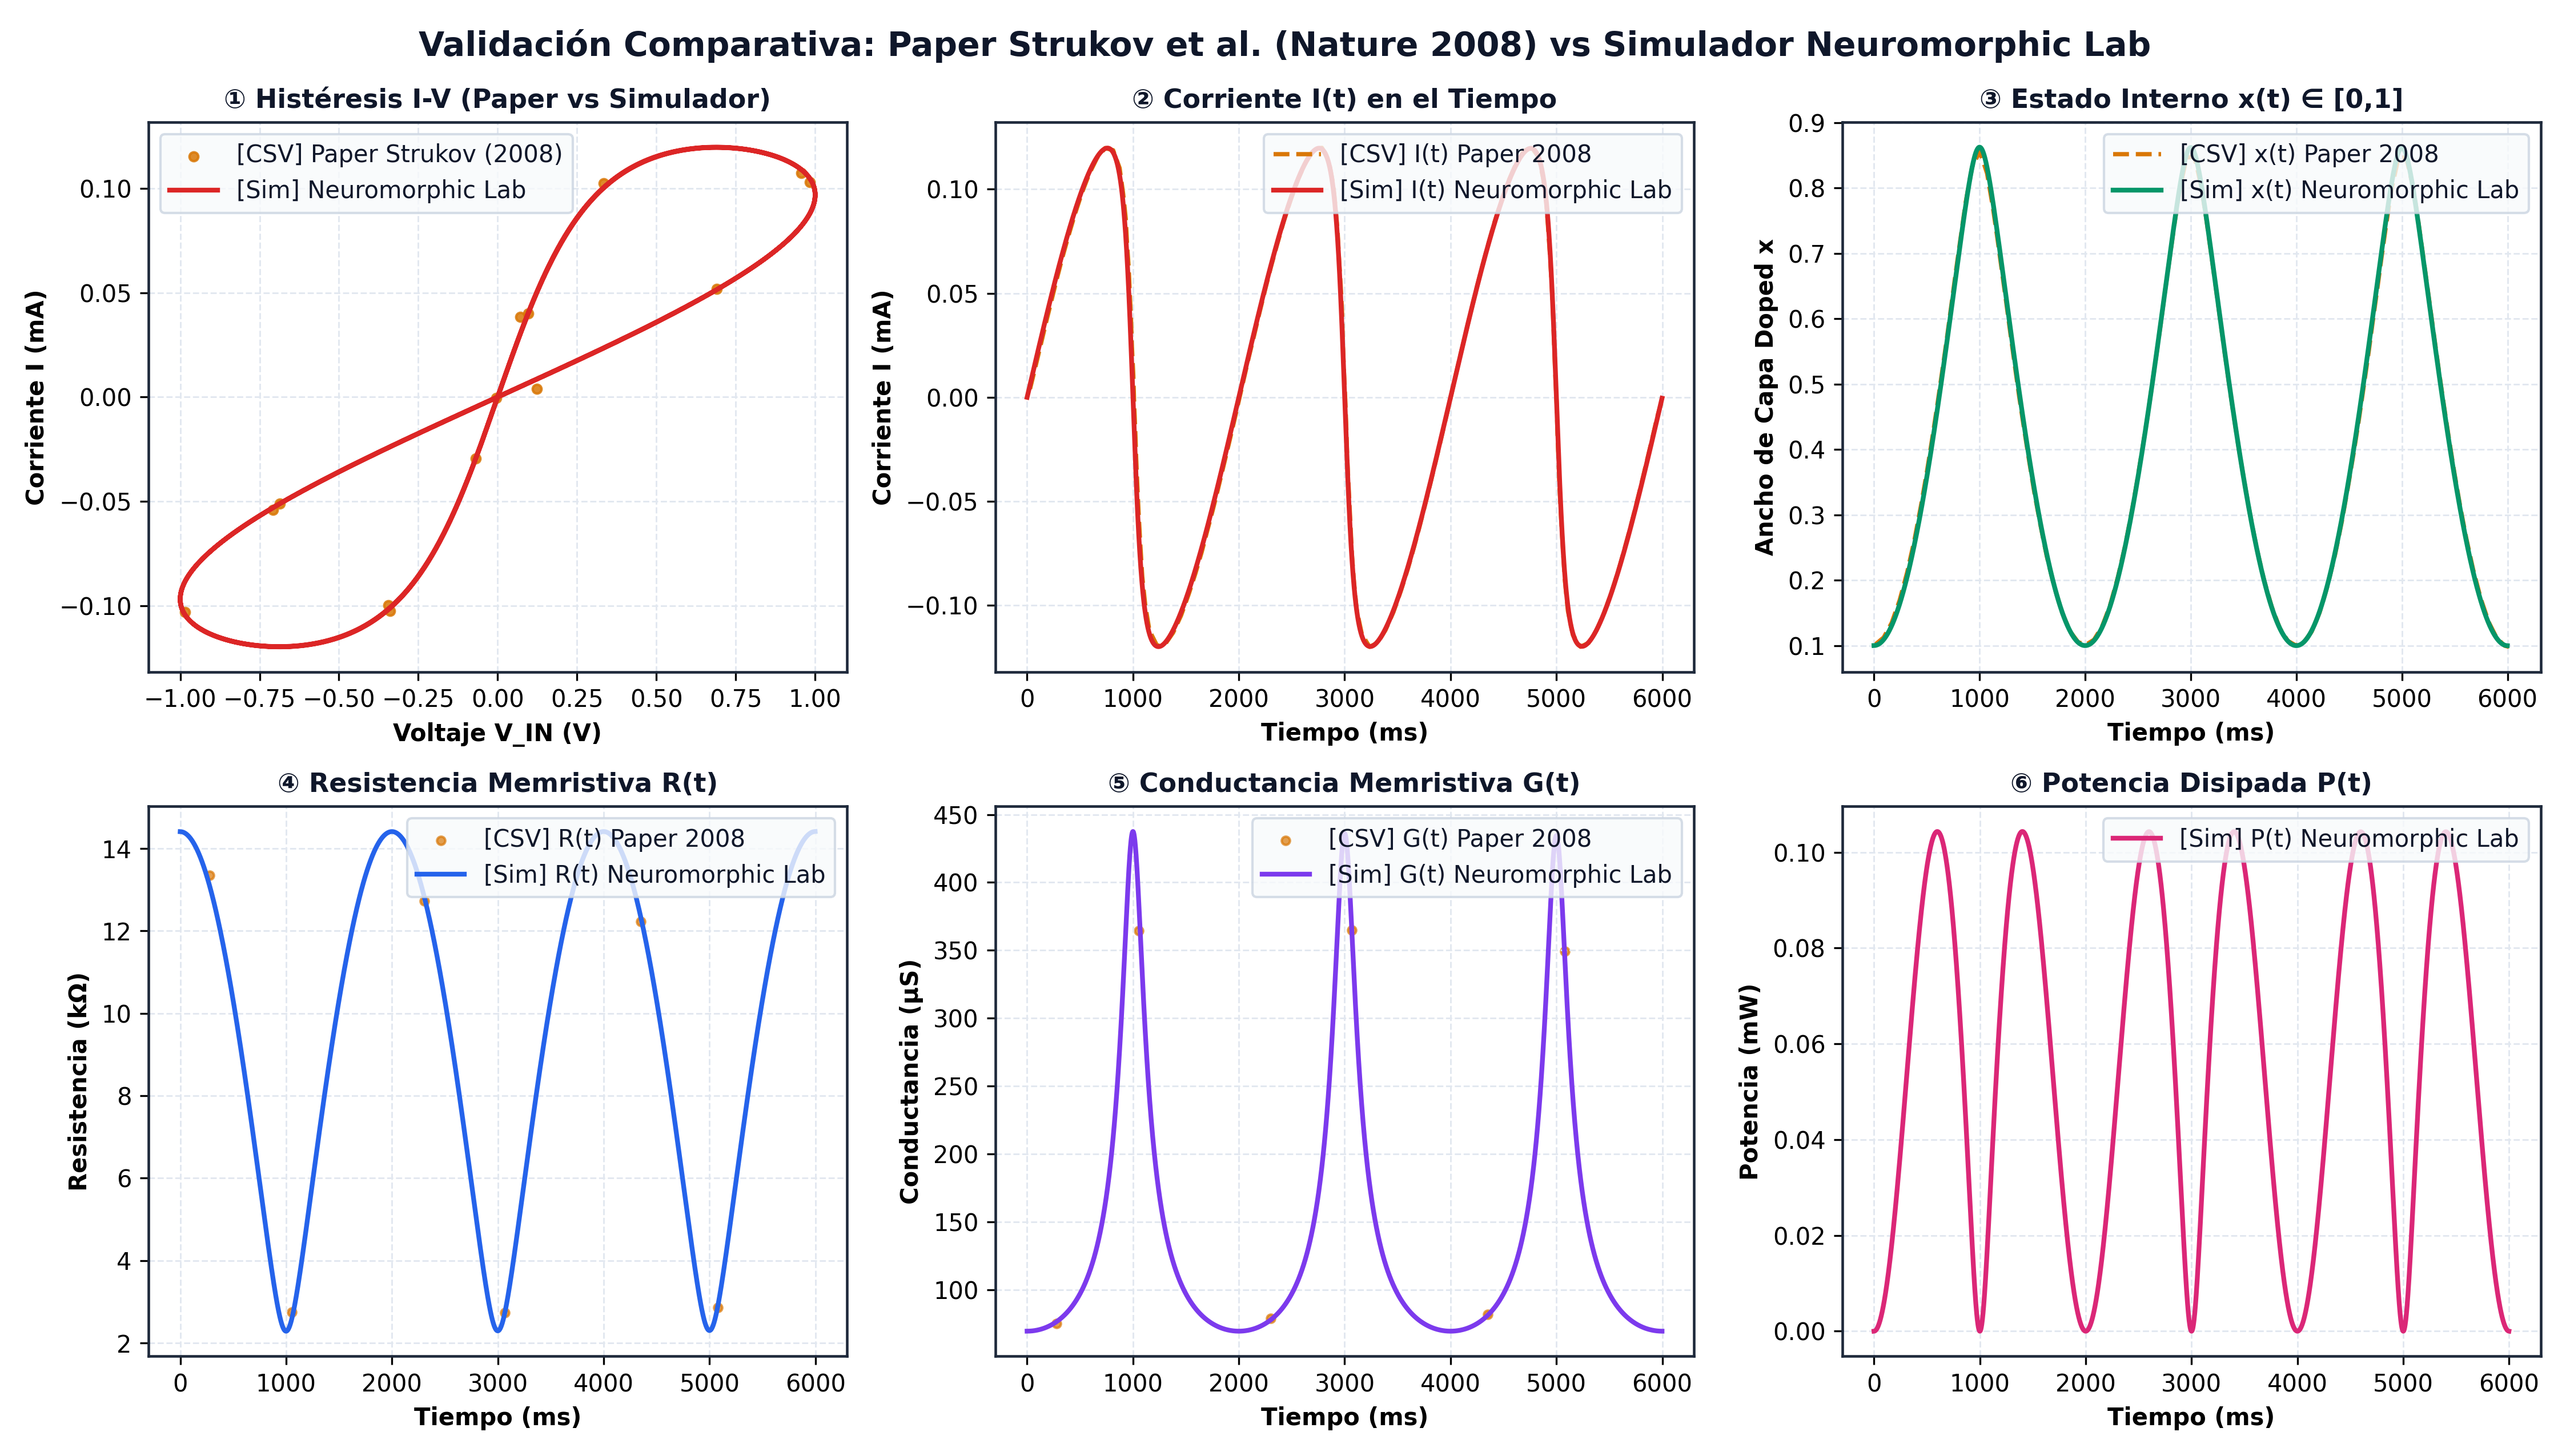
\includegraphics[width=\textwidth]{figuras/validacion_memristor.png}
\caption{Validación cuantitativa de los modelos memristivos 
implementados. Izquierda: lazo de histéresis del modelo de 
Strukov contra datos de Nature 2008. Derecha: asimetría 
SET/RESET del modelo de Prezioso contra datos de Nature 
Communications 2014.}
\label{fig:validacion_memristor}
\end{figure}

Sobre el modelo de Strukov se incorporaron tres fuentes de 
variabilidad estocástica: variabilidad dispositivo a dispositivo 
(D2D) mediante distribuciones normales truncadas sobre los 
parámetros eléctricos, variabilidad ciclo a ciclo (C2C) mediante 
un proceso de Ornstein-Uhlenbeck inyectado en la derivada 
temporal del estado, y ruido térmico modelado como ruido 
gaussiano blanco superpuesto al voltaje de entrada. La 
Figura~\ref{fig:variabilidad} presenta la caracterización 
estadística de ambos tipos de variabilidad.

\begin{figure}[H]
\centering
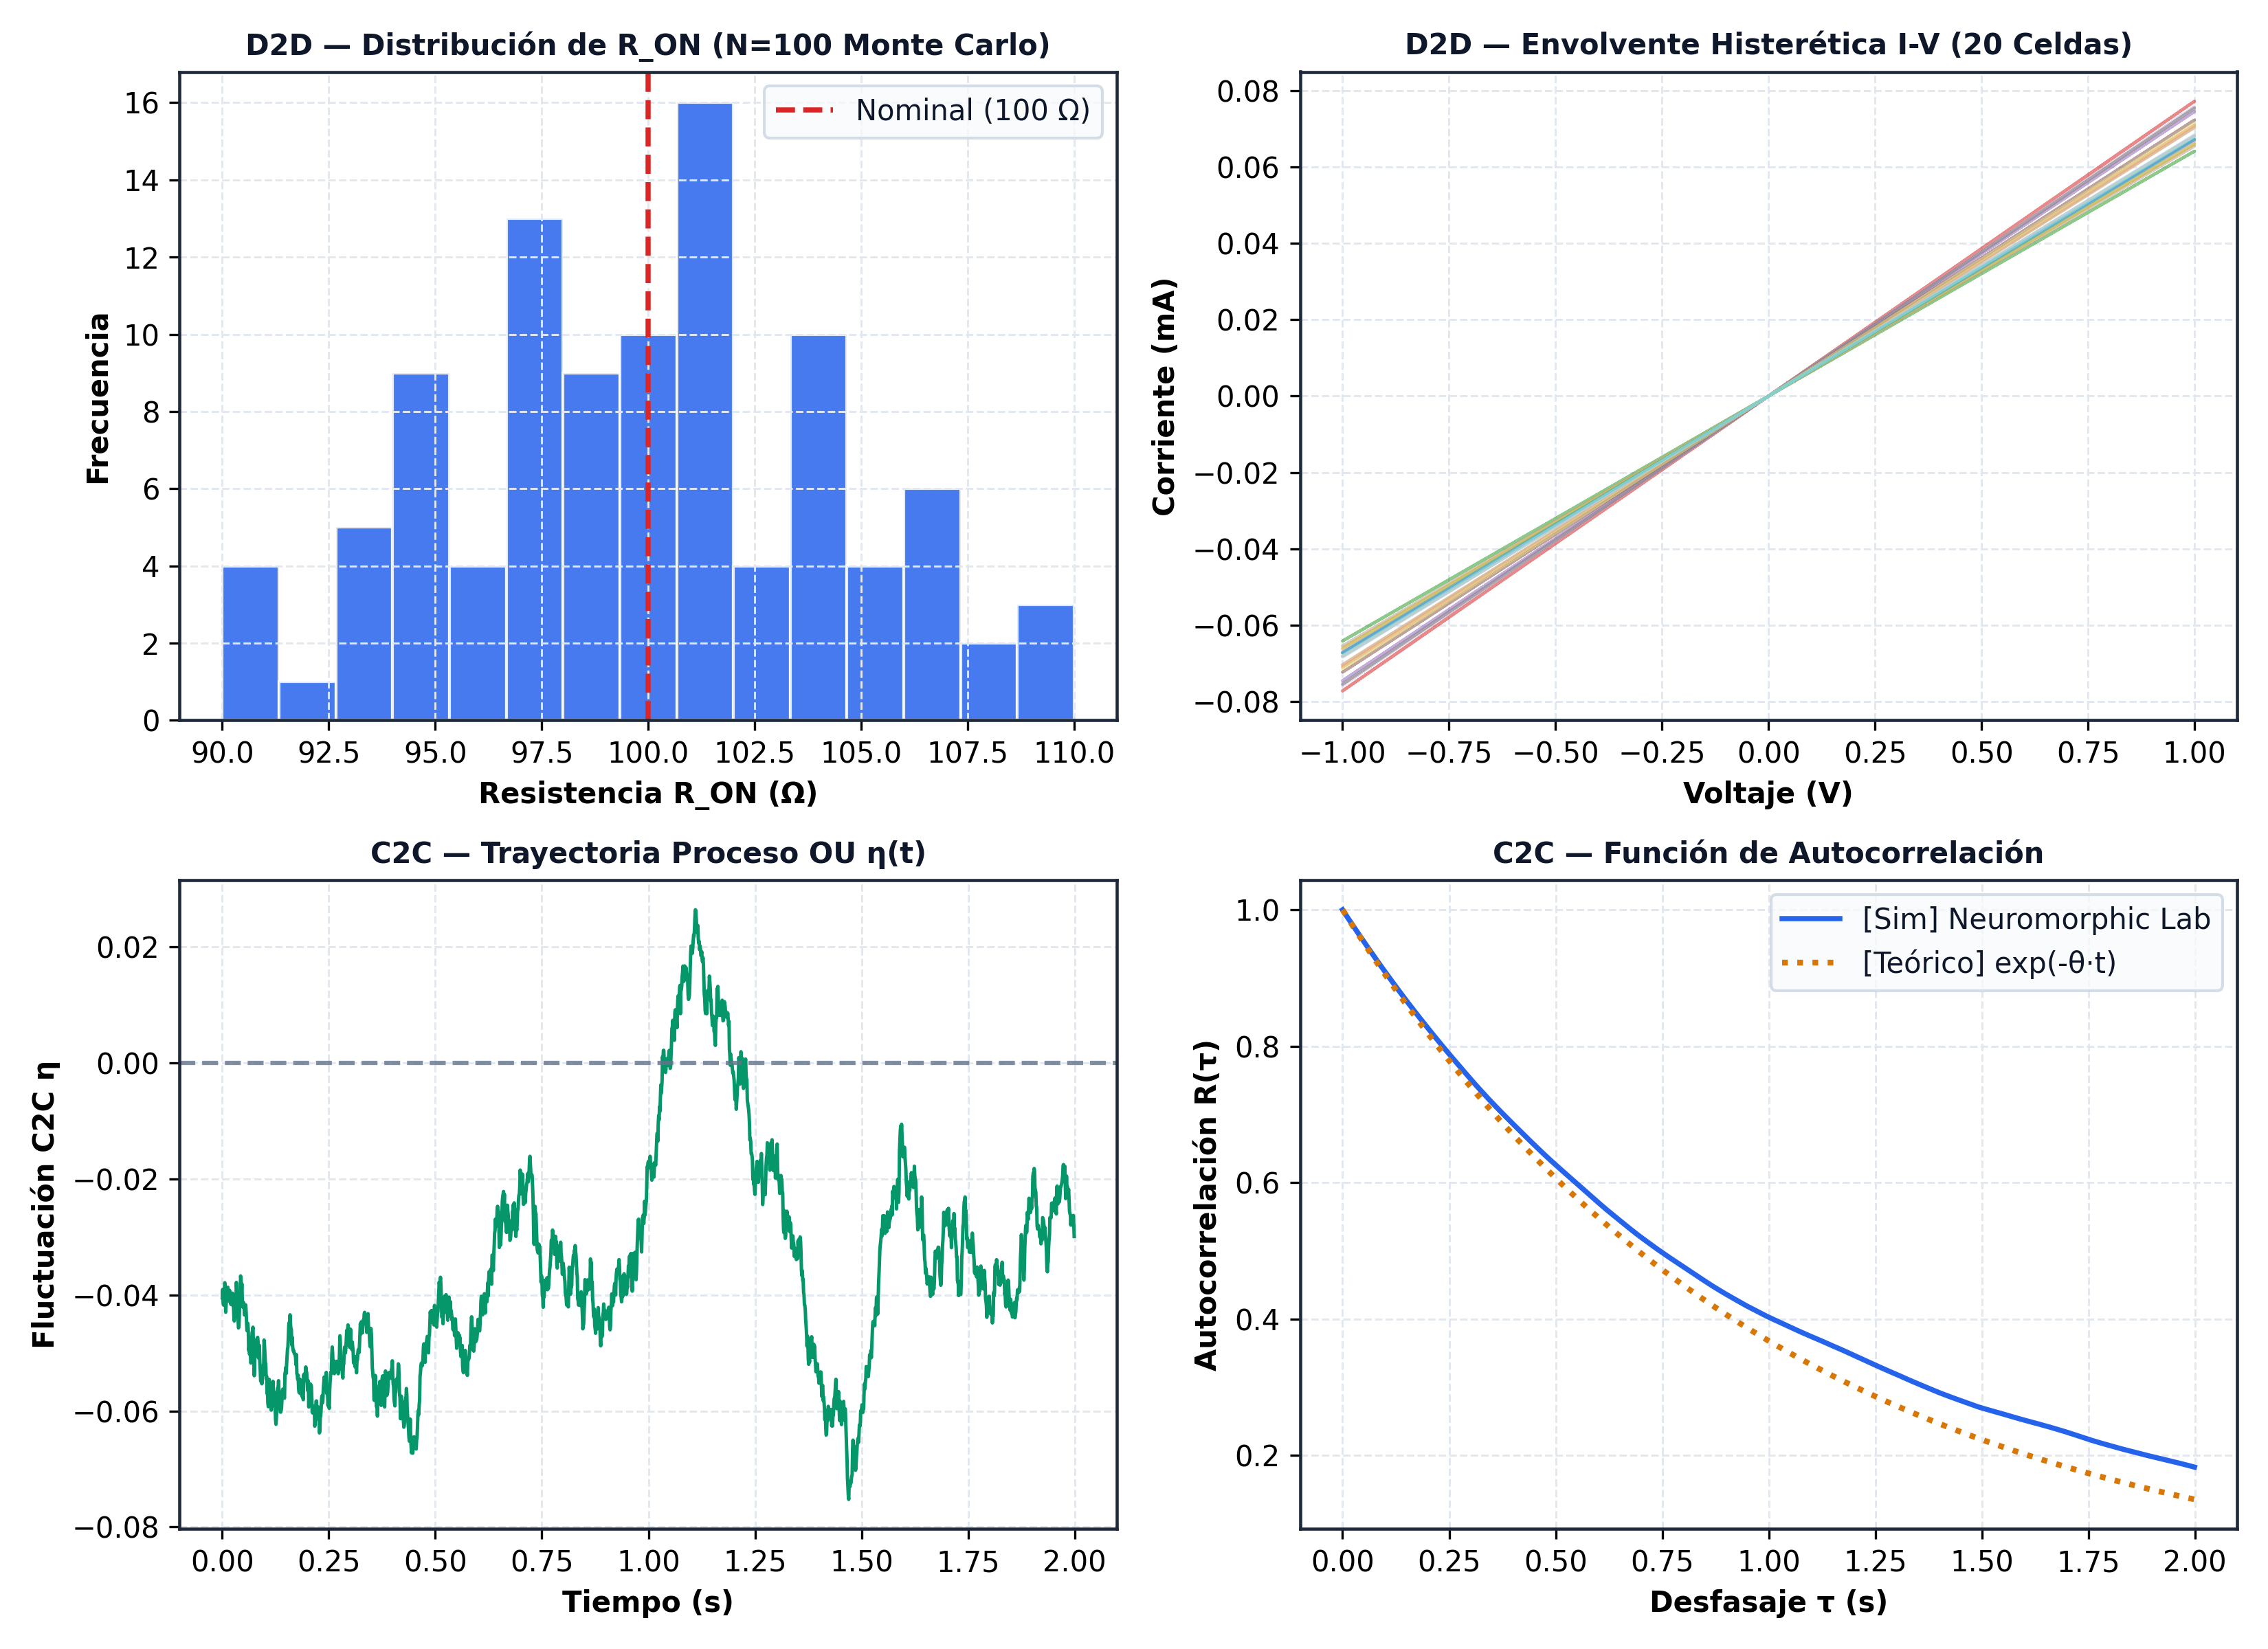
\includegraphics[width=\textwidth]{figuras/variabilidad_d2d_c2c.png}
\caption{Caracterización cuantitativa de variabilidad D2D 
(histograma de $R_{ON}$ con ajuste normal) y variabilidad 
temporal C2C (trayectoria del proceso de Ornstein-Uhlenbeck y 
función de autocorrelación).}
\label{fig:variabilidad}
\end{figure}

\subsection{Etapa 2 -- Neurona LIF y sistema híbrido}

Se implementó una neurona tipo Leaky Integrate-and-Fire (LIF) 
como bloque de procesamiento neuronal. El potencial de membrana 
se modela como el voltaje de un capacitor $C_m$ sujeto a una 
corriente de fuga a través de una resistencia $R_{leak}$, con 
una resistencia en serie $R_{series}$ que limita la corriente 
de entrada. Cuando el potencial cruza el umbral $V_{th}$, la 
neurona emite un pulso y reinicia su estado, entrando en un 
período refractario absoluto.

El acoplamiento memristor--neurona se implementó en configuración 
serie: el memristor sustituye la resistencia de entrada de la 
neurona, de modo que la corriente inyectada depende del estado 
interno $x(t)$ del dispositivo. El resultado es una modulación 
dinámica de la frecuencia de disparo: conforme el memristor 
reduce su resistencia, la neurona dispara más rápido, 
reproduciendo el comportamiento de adaptación sensorial 
observado en neuronas biológicas.

La Figura~\ref{fig:lif_analitica} valida el integrador numérico 
de la LIF contra la solución analítica exacta del circuito RC 
subumbral, alcanzando un coeficiente de determinación 
$R^2 = 1.0000$.

\begin{figure}[H]
\centering
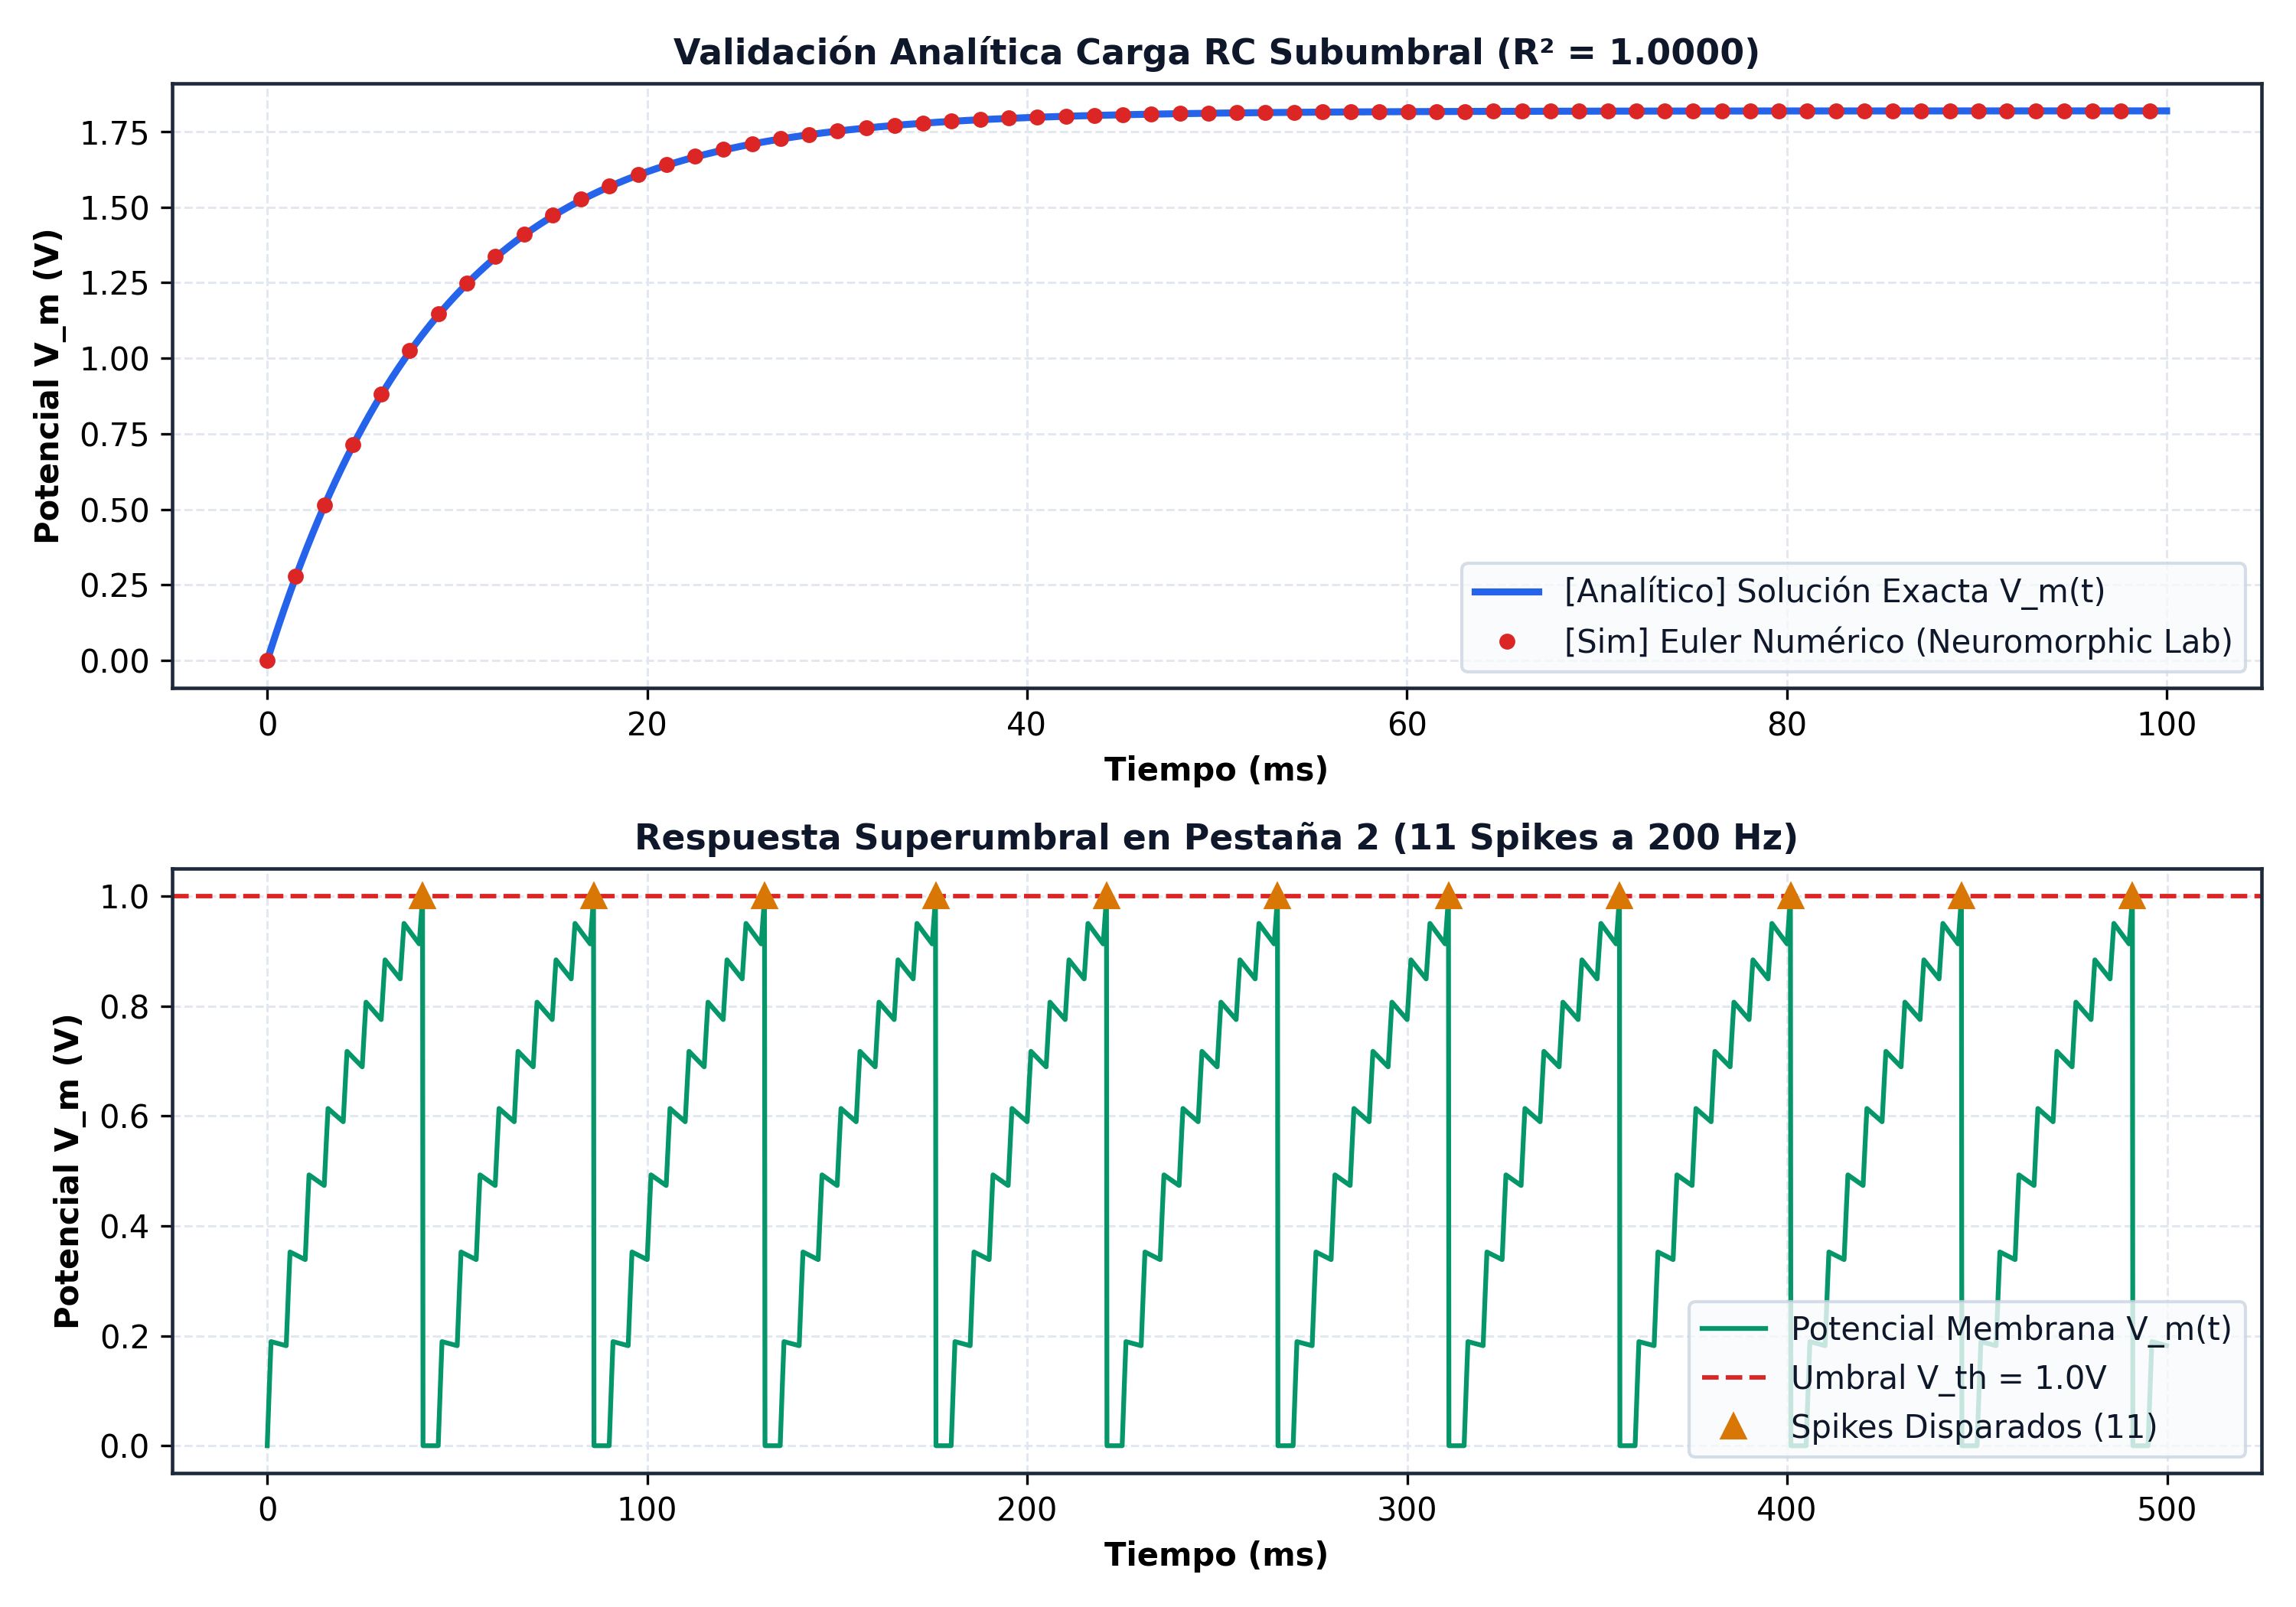
\includegraphics[width=\textwidth]{figuras/lif_analitica.png}
\caption{Validación analítica subumbral de la neurona LIF. 
Panel superior: solución exacta (azul) contra integración 
Euler (marcadores). Panel inferior: respuesta supraliminal 
con tren de pulsos.}
\label{fig:lif_analitica}
\end{figure}

La Figura~\ref{fig:sistema_hibrido} presenta la respuesta del 
sistema híbrido completo con un memristor volátil de HfO$_2$. 
Al aplicar un estímulo constante, el memristor reduce su 
resistencia, la corriente inyectada aumenta y el intervalo 
inter-spike se comprime. Al cesar el estímulo, el memristor 
se relaja espontáneamente y la neurona vuelve a su régimen 
basal.

\begin{figure}[H]
\centering
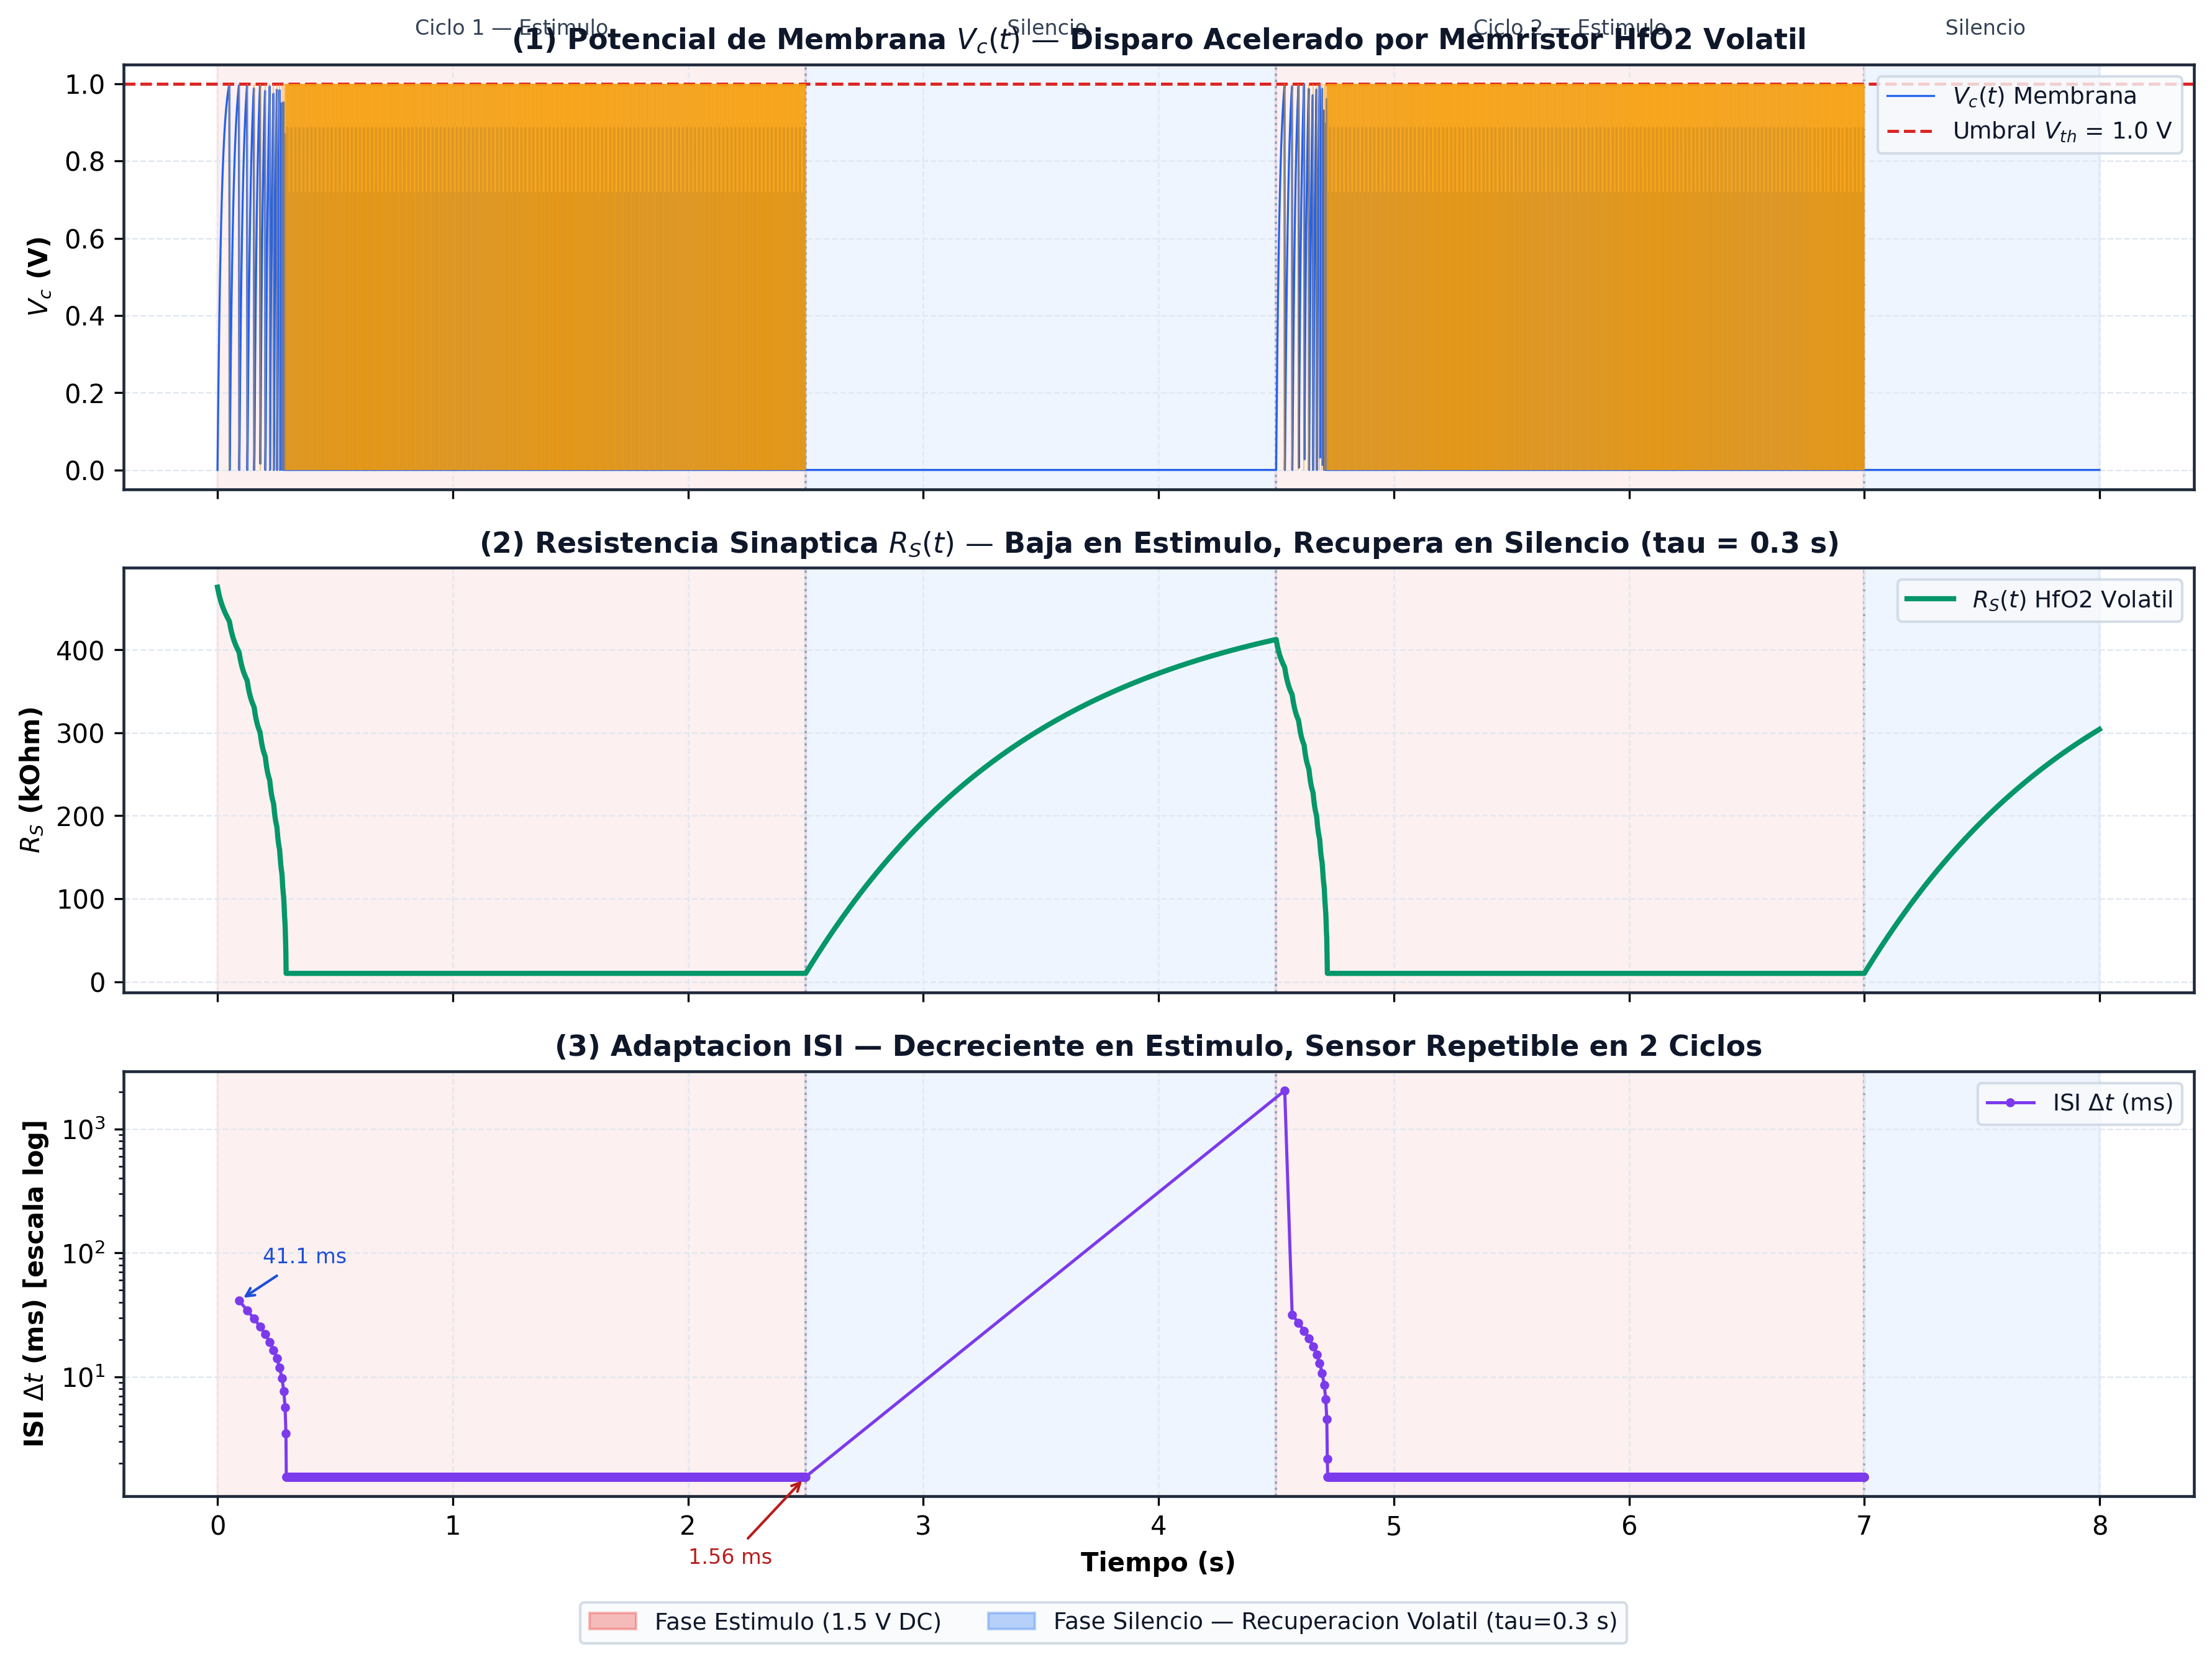
\includegraphics[width=\textwidth]{figuras/sistema_hibrido.png}
\caption{Respuesta del sistema híbrido memristor--neurona. 
Panel superior: potencial de membrana. Panel central: 
resistencia sináptica. Panel inferior: intervalo inter-spike 
en escala logarítmica.}
\label{fig:sistema_hibrido}
\end{figure}

La repetibilidad del sistema se verificó aplicando dos ciclos 
consecutivos de estímulo y silencio. La diferencia en el número 
total de pulsos entre ambos ciclos fue inferior al 0.3\%, 
evidenciando que el memristor retorna espontáneamente a su 
estado inicial tras el cese de la excitación.

\subsection{Etapa 3 -- Plasticidad sináptica}

Sobre el modelo memristivo se implementaron dos reglas de 
plasticidad sináptica: potenciación y depresión a largo plazo 
(LTP/LTD) mediante secuencias de pulsos, y plasticidad 
dependiente del tiempo de disparo (STDP) mediante solapamiento 
temporal de espigas.

La regla LTP/LTD modifica la conductancia del dispositivo de 
forma gradual: pulsos positivos incrementan la conductancia 
(LTP), mientras que pulsos negativos la reducen (LTD). La 
evolución de la conductancia presenta saturación asintótica 
en los límites $G_{max}$ y $G_{min}$, reproduciendo la no 
linealidad observada en dispositivos reales. Tras 100 ciclos 
consecutivos de conmutación extrema, el dispositivo retorna a 
su estado inicial con un error acumulado inferior al 1\%, 
evidenciando ausencia de deriva (drift).

La regla STDP se implementó siguiendo la arquitectura de 
solapamiento de espigas formalizada por Jo et al. (2010). Un 
evento de cambio conductivo solo ocurre cuando una espiga 
pre-sináptica y una post-sináptica convergen temporalmente, 
generando un diferencial de voltaje trans-memristivo que 
excede el umbral de programación. El signo del desfase 
temporal $\Delta t$ determina el régimen: potenciación si 
$\Delta t > 0$ (pre antes de post) y depresión si 
$\Delta t < 0$ (post antes de pre).

La Figura~\ref{fig:ltp_ltd} presenta la evolución de la 
conductancia bajo secuencias de pulsos LTP/LTD. La 
Figura~\ref{fig:stdp} valida la ventana STDP bi-exponencial 
contra los puntos experimentales digitalizados de Jo et al. 
(2010), alcanzando $R^2 = 0.9678$ y un error absoluto medio 
de 1.30\%.

\begin{figure}[H]
\centering
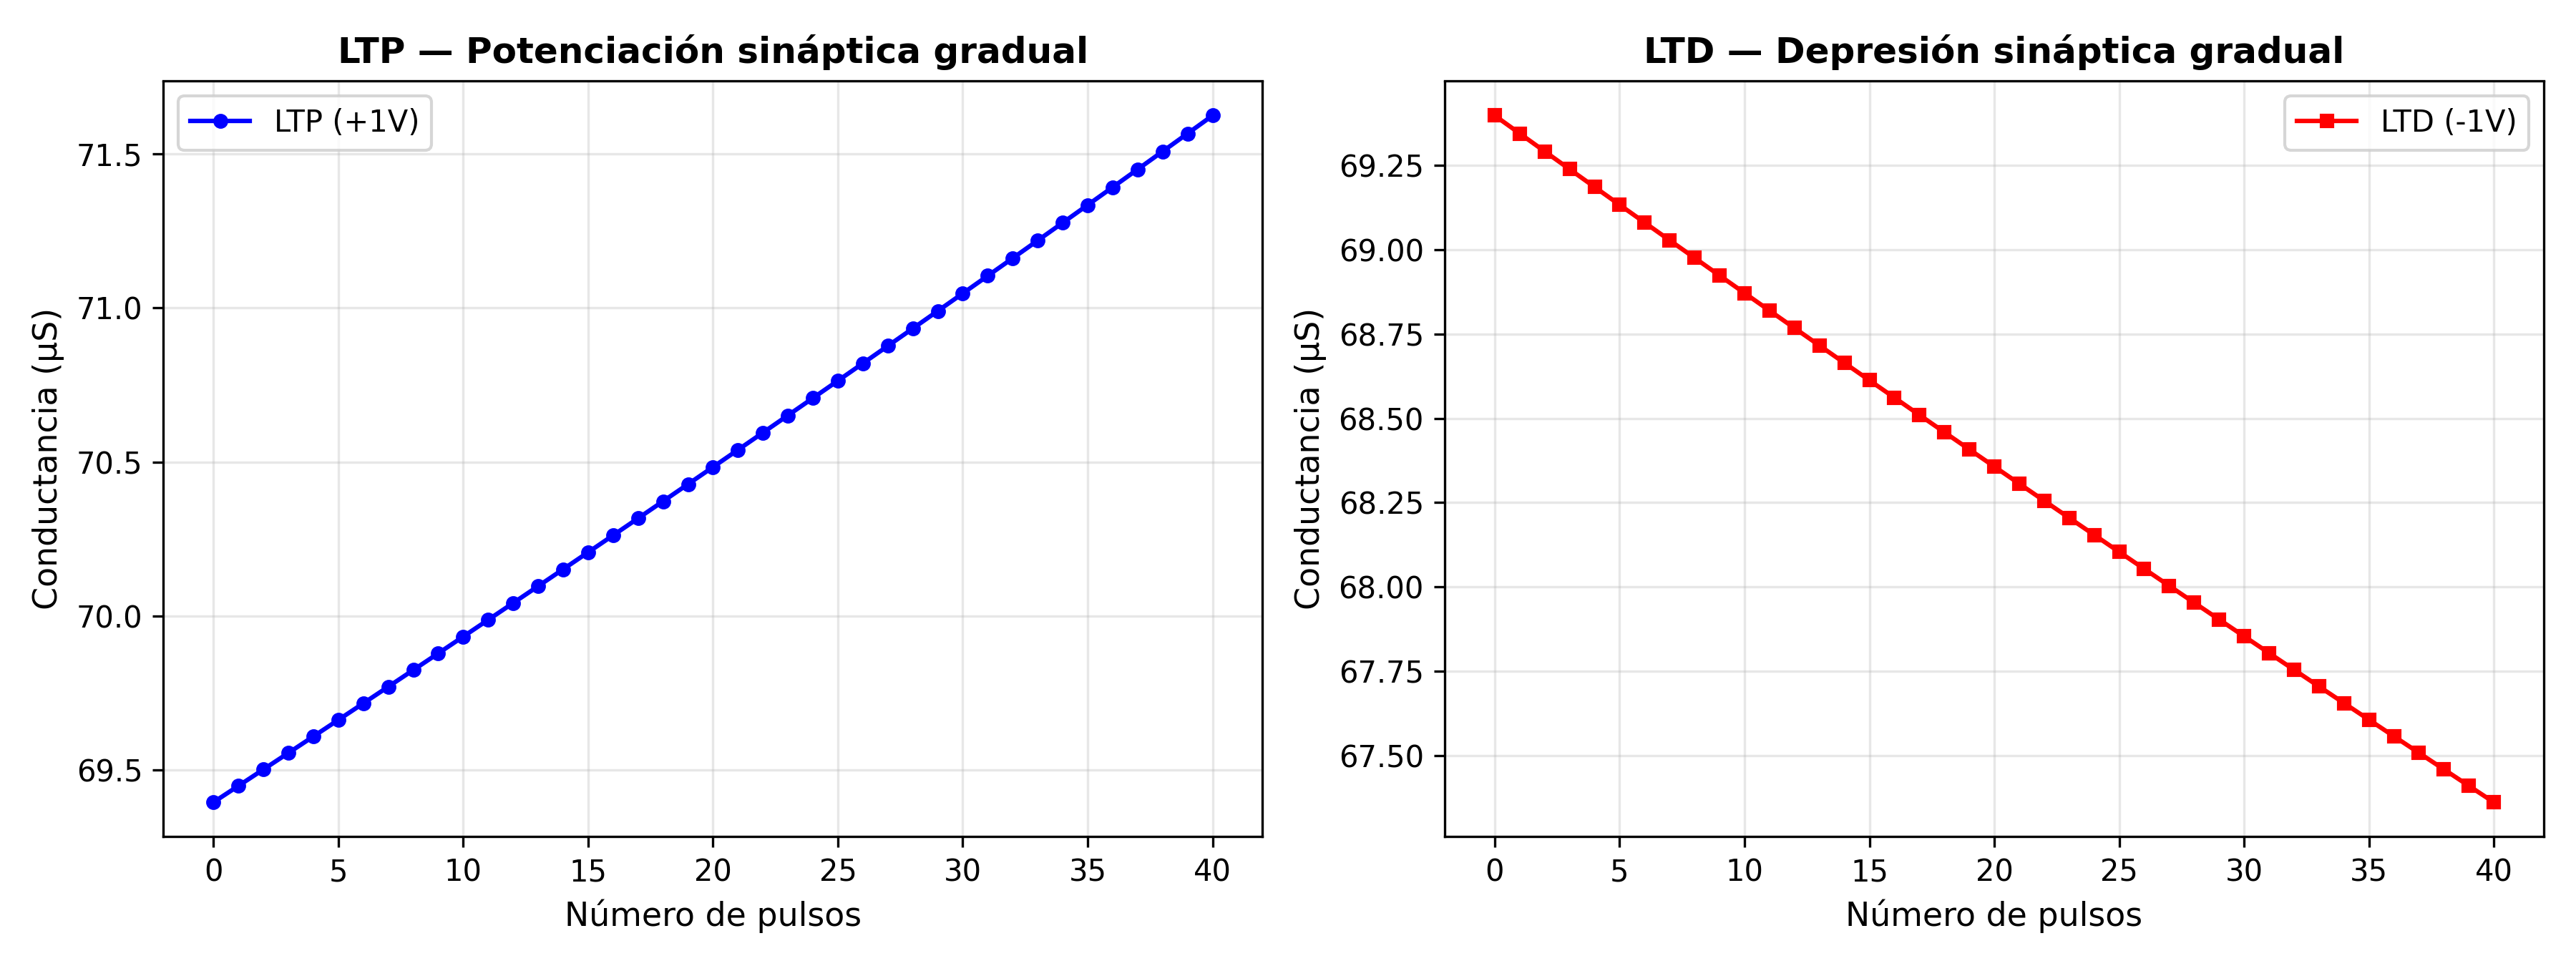
\includegraphics[width=\textwidth]{figuras/ltp_ltd.png}
\caption{Implementación cualitativa de LTP y LTD mediante 
secuencias continuas de pulsos idénticos. La conductancia se 
modifica de forma gradual con saturación asintótica en los 
extremos.}
\label{fig:ltp_ltd}
\end{figure}

\begin{figure}[H]
\centering
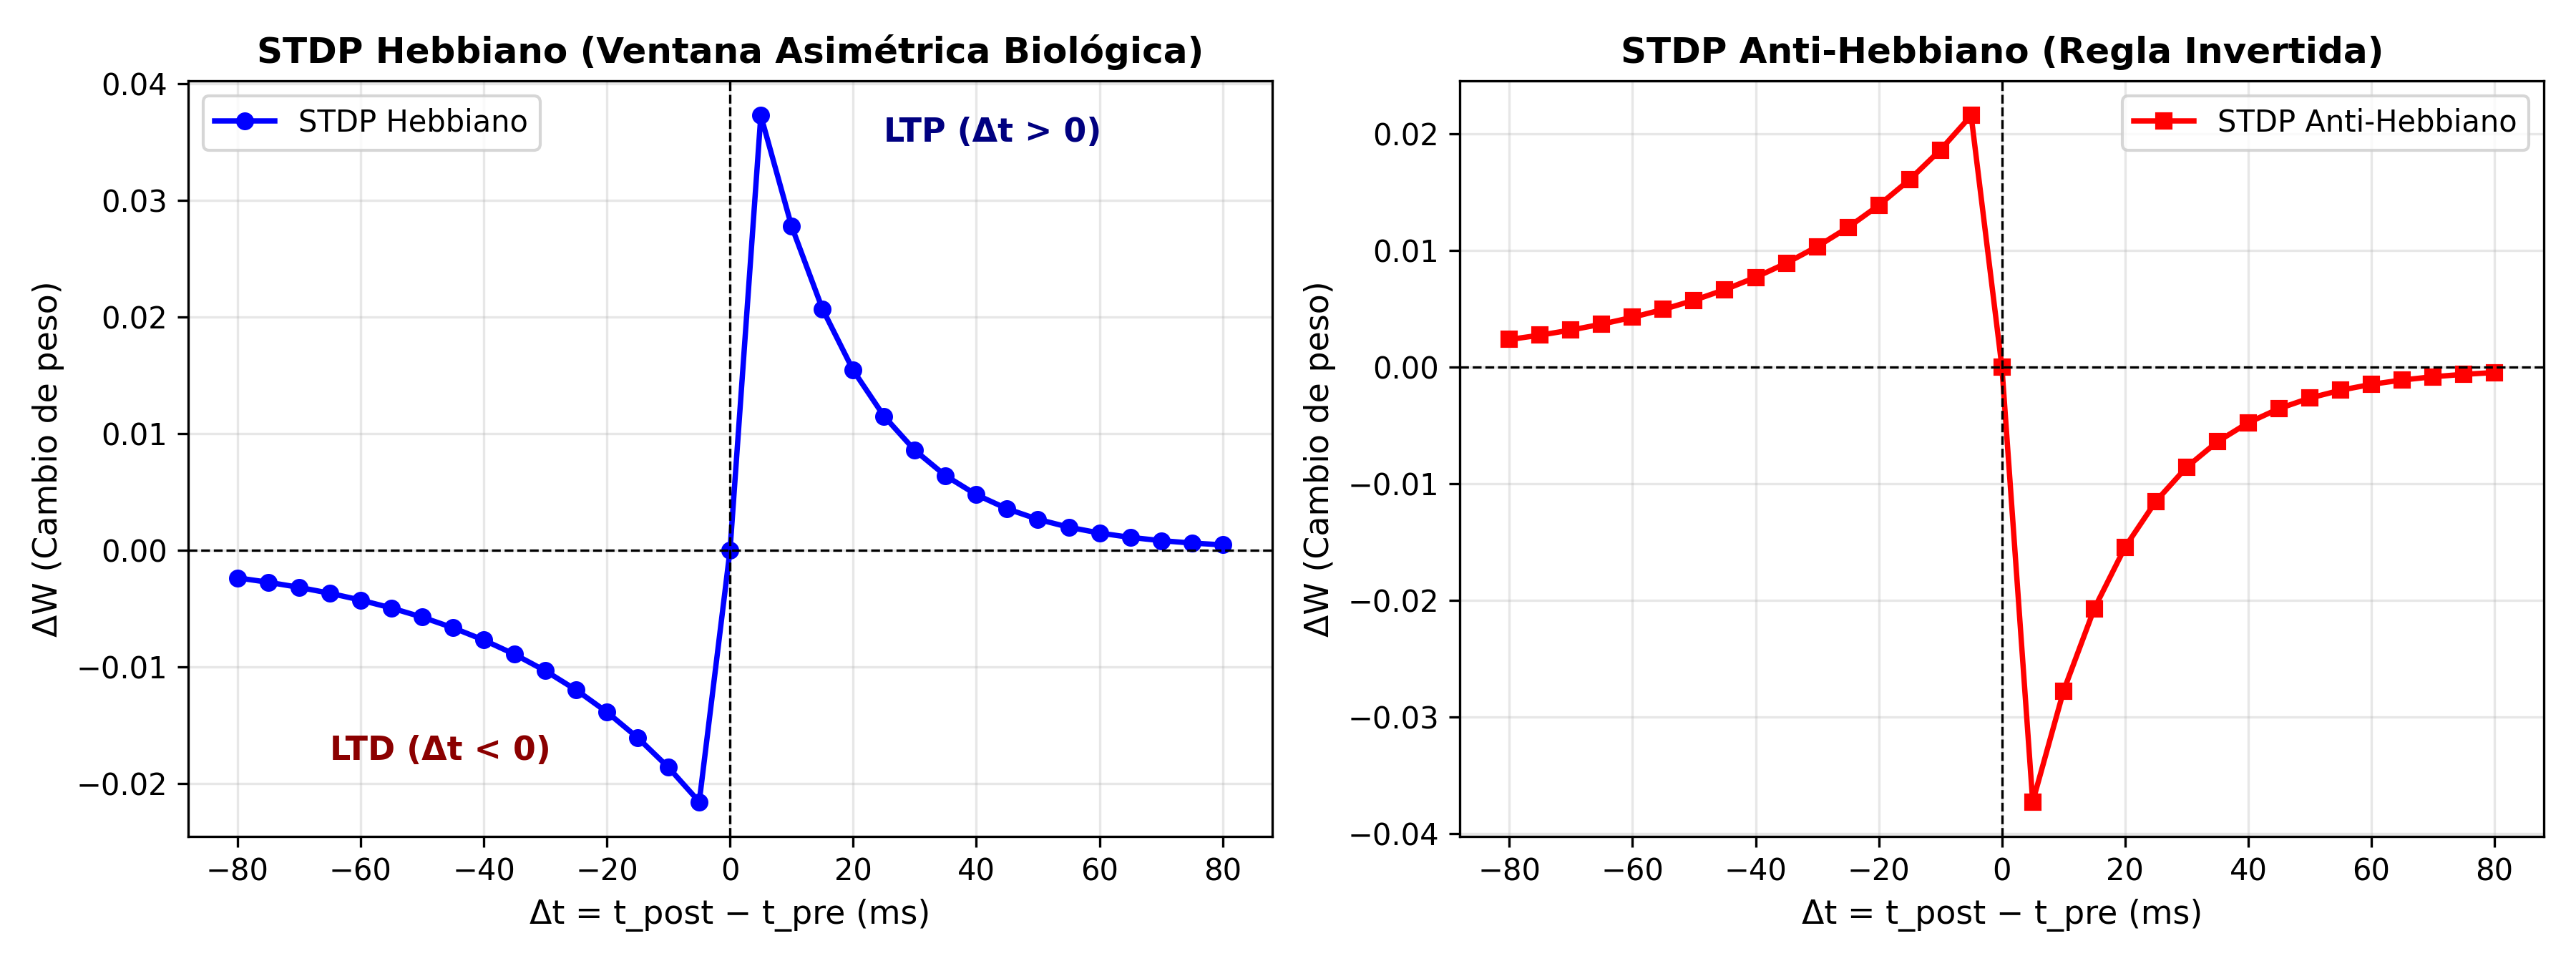
\includegraphics[width=\textwidth]{figuras/stdp.png}
\caption{Validación cuantitativa de la ventana STDP 
bi-exponencial contra los puntos experimentales de Jo et al. 
(2010). Modelo analítico (línea verde) contra datos discretos 
(marcadores rojos y azules).}
\label{fig:stdp}
\end{figure}

\subsection{Etapa 4 -- Crossbar e in-memory computing}

Los dispositivos memristivos individuales se organizaron en 
arreglos matriciales de tipo crossbar $N \times M$, donde cada 
intersección aloja un dispositivo cuya conductancia representa un 
peso sináptico. Esta arquitectura permite realizar operaciones de 
multiplicación vector-matriz directamente sobre el hardware, 
aprovechando las leyes de Ohm y Kirchhoff en lugar de cómputo 
digital secuencial.

La corriente integrada por cada columna $j$ se obtiene resolviendo 
un sistema nodal completo sobre la topología del arreglo. A 
diferencia de los modelos matriciales idealizados, el solver 
incorpora resistencias de línea $R_{wire}$ entre celdas adyacentes, 
impedancias de sensado $R_{sense}$ en las columnas, e impedancias 
de driver en las filas. El resultado es una matriz de nodos de 
dimensión $2NM \times 2NM$ que se resuelve mediante análisis nodal 
modificado (MNA).

Este enfoque captura de forma natural dos efectos no ideales que 
los simuladores de software tradicionales suelen omitir. En primer 
lugar, las corrientes parásitas o \textit{sneak paths}: rutas 
alternativas de corriente que degradan la precisión de lectura y 
que crecen con el tamaño del arreglo. En segundo lugar, las caídas 
de voltaje por resistencia de línea (IR drops), que distorsionan 
el perfil de corriente a lo largo de cada columna.

La Figura~\ref{fig:sneak_ratio} cuantifica el crecimiento del 
sneak ratio en función del tamaño del arreglo, desde $N=4$ hasta 
$N=32$ filas. La Figura~\ref{fig:mna_vs_ideal} compara las 
corrientes obtenidas por el solver MNA contra el modelo ideal 
$I = G \cdot V$, evidenciando que el error relativo alcanza el 
3.63\% para $N=24$.

\begin{figure}[H]
\centering
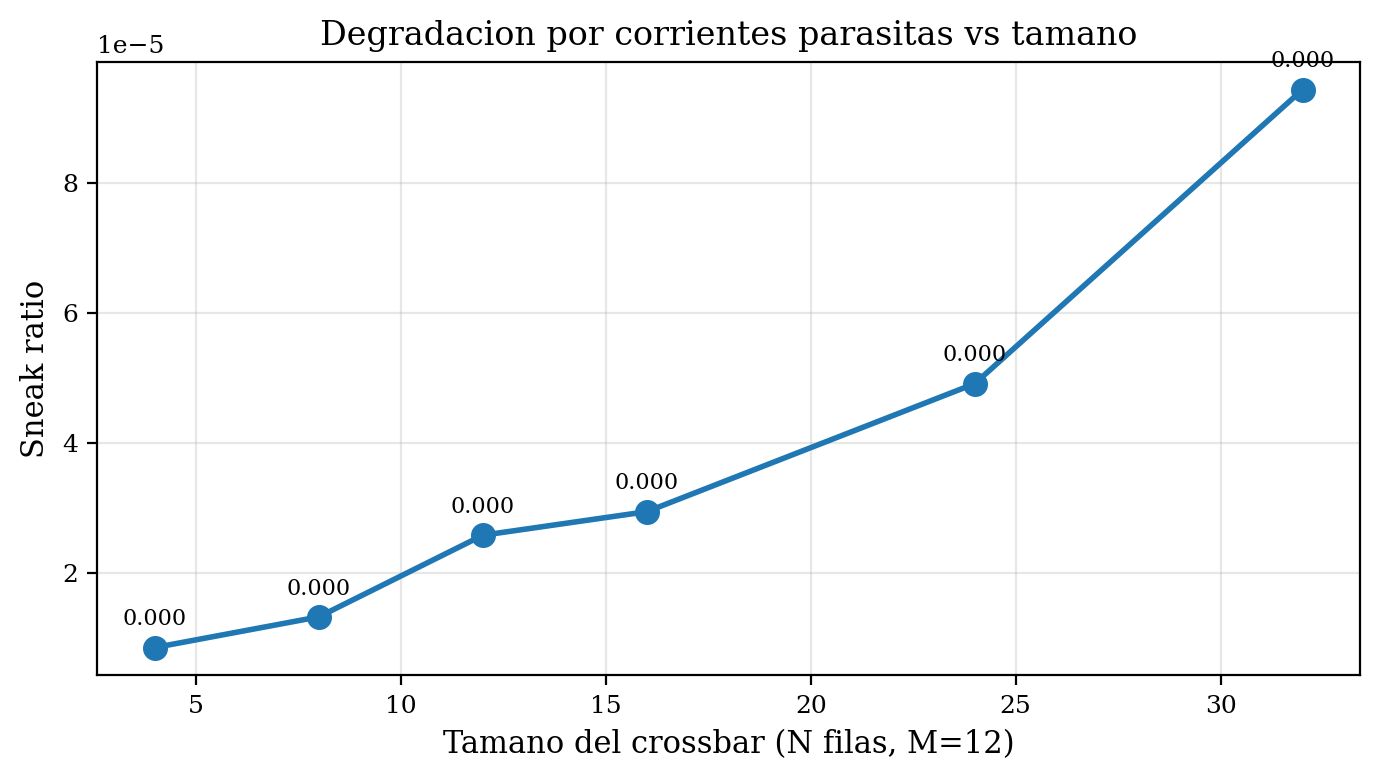
\includegraphics[width=0.75\textwidth]{figuras/sneak_ratio_vs_N.png}
\caption{Crecimiento monótono del sneak ratio al escalar el 
arreglo crossbar desde $N=4$ hasta $N=32$ filas, con $M=12$ 
columnas fijas.}
\label{fig:sneak_ratio}
\end{figure}

\begin{figure}[H]
\centering
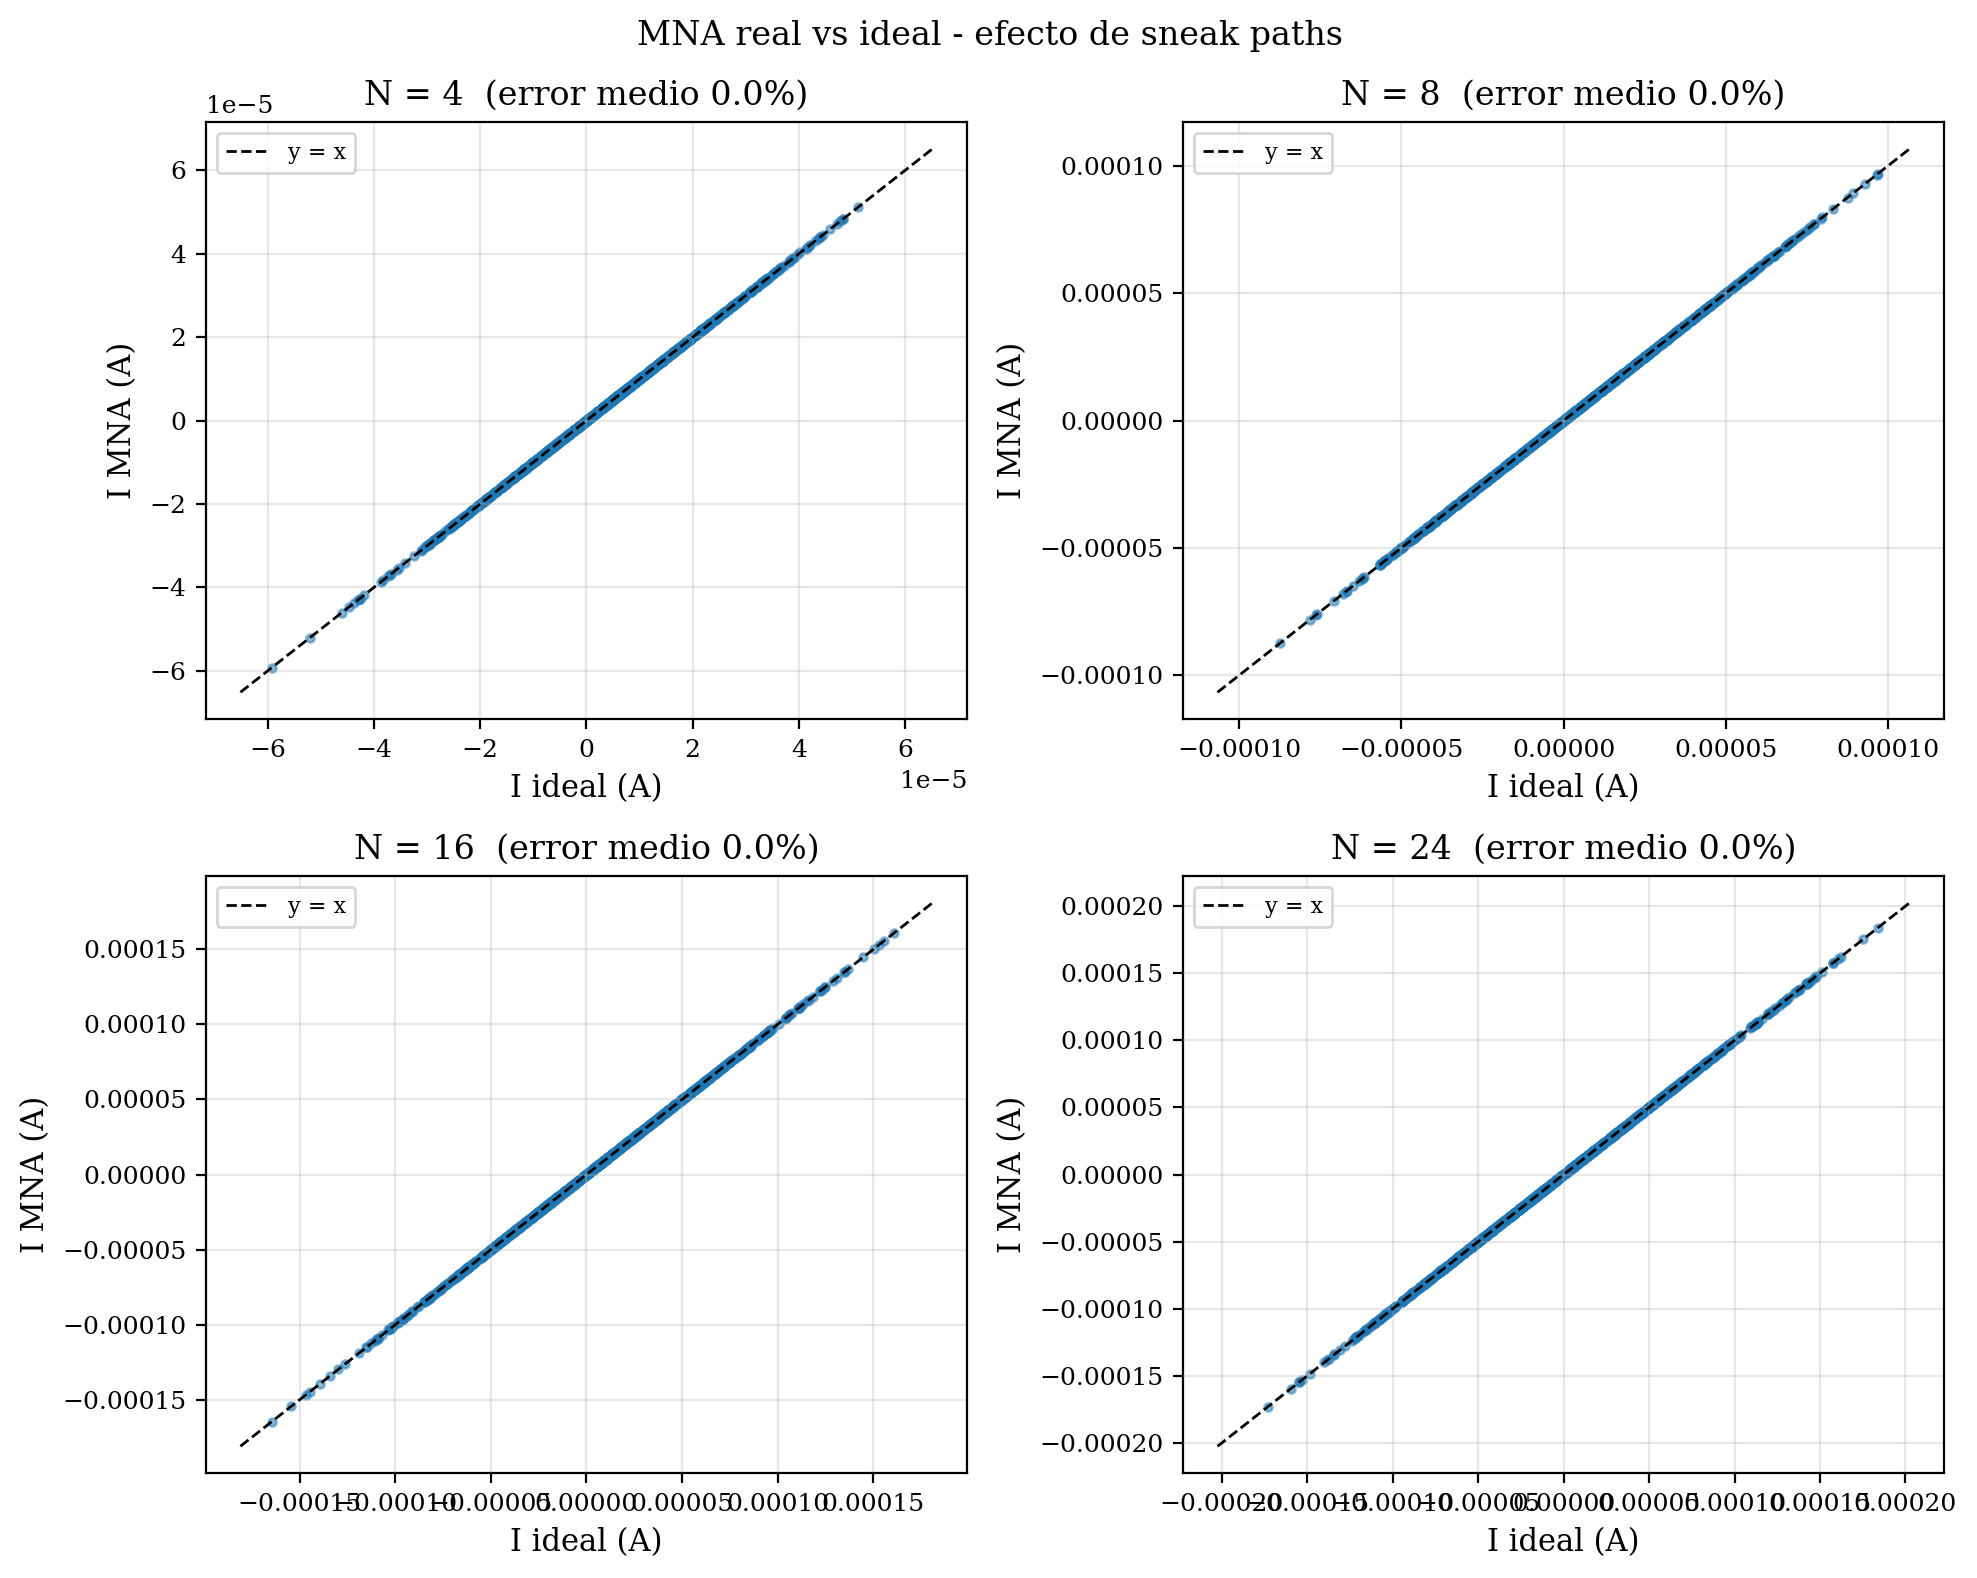
\includegraphics[width=\textwidth]{figuras/mna_vs_ideal.png}
\caption{Comparación entre corrientes calculadas por el solver 
MNA completo y el modelo ideal $I = G \cdot V$ para cuatro 
tamaños de arreglo. La desviación respecto a la recta identidad 
refleja el impacto acumulado de las corrientes parásitas.}
\label{fig:mna_vs_ideal}
\end{figure}

La Figura~\ref{fig:ir_drops} ilustra el efecto de la resistencia 
de línea sobre el perfil de corriente: para $R_{wire} \geq 1\,\Omega$, 
las variaciones entre columnas alcanzan el $\pm 30\%$. Este 
resultado motiva el uso de esquemas de escritura asimétricos como 
$V/2$ y $V/3$, que reducen la perturbación de celdas half-selected 
durante operaciones de programación.

\begin{figure}[H]
\centering
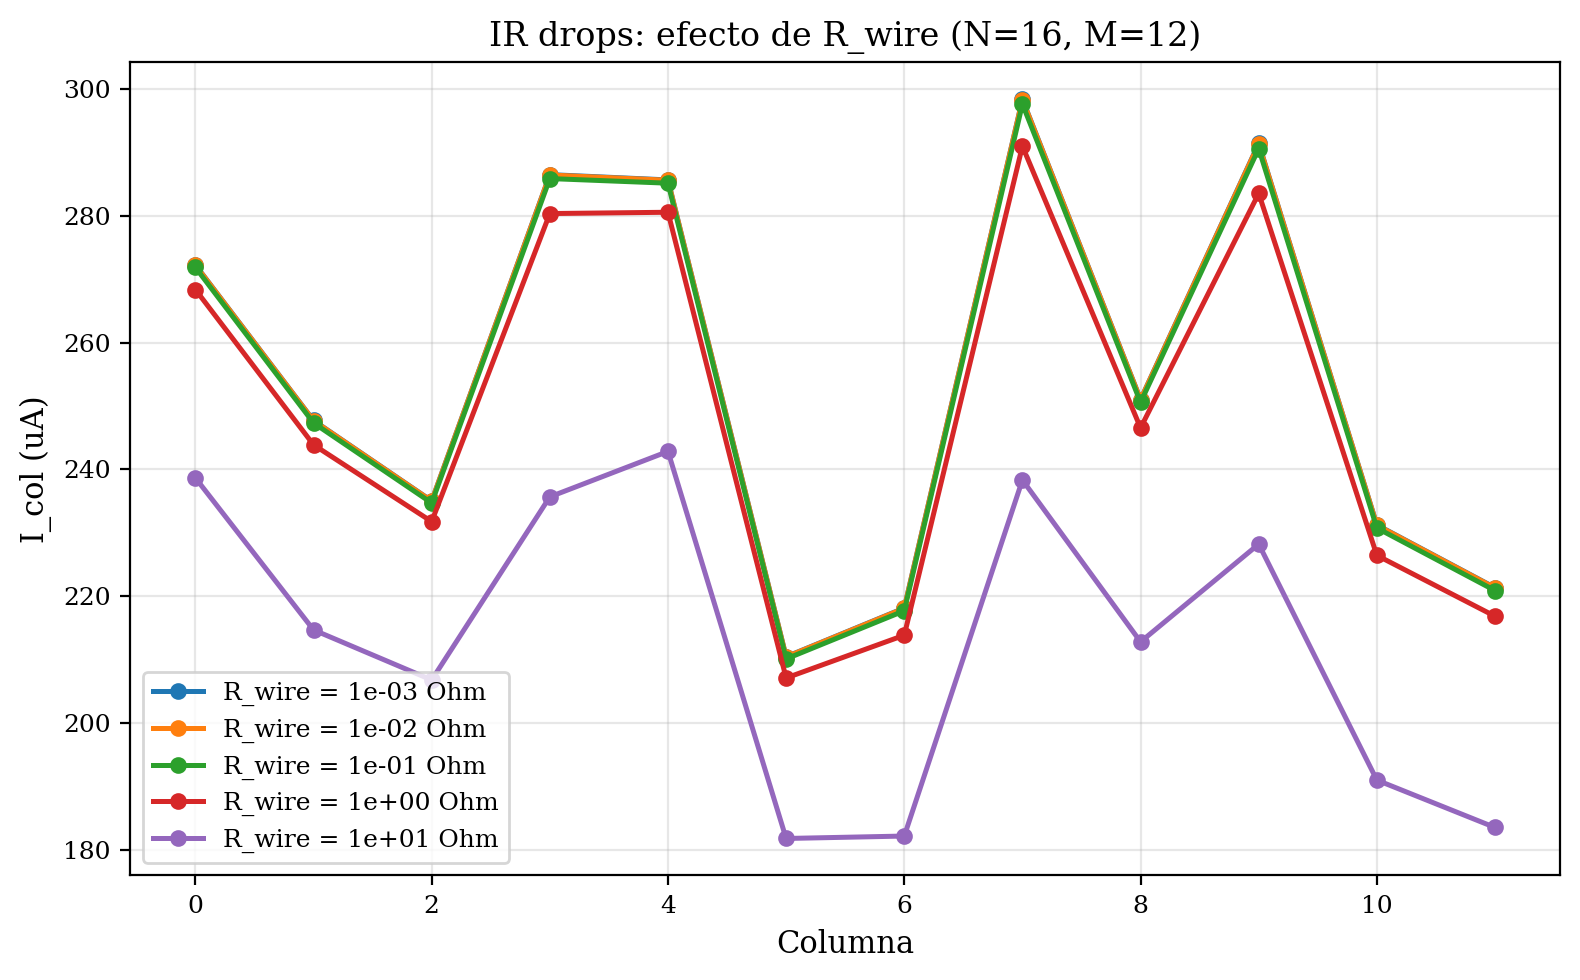
\includegraphics[width=0.75\textwidth]{figuras/ir_drops.png}
\caption{Perfil de corriente por columna para distintos valores 
de resistencia de línea $R_{wire}$. A mayor resistencia, mayor 
no-uniformidad en la lectura.}
\label{fig:ir_drops}
\end{figure}
\subsection{Etapa 5 -- Integración con agente de control autónomo}

Los componentes anteriores se integraron en un agente de 
control cuyo sustrato físico es el propio arreglo crossbar. El 
agente opera en un ciclo de cuatro etapas: codificación 
sensorial, propagación analógica por el crossbar, decodificación 
estocástica de la acción, y actualización de pesos al final del 
episodio.

\subsubsection{Codificación sensorial}

El vector de observación del entorno se proyecta sobre las 
filas del crossbar mediante un codificador unipolar con 
selección top-$k$. Cada componente de la observación se 
combina linealmente con un banco de pesos fijos, generando un 
conjunto de activaciones. Se seleccionan las $k$ filas con mayor 
respuesta y se aplican voltajes de lectura, mientras el resto 
permanece inactivo. Este esquema produce una representación 
dispersa y mantiene los voltajes por debajo del umbral de 
escritura, garantizando lectura no destructiva.

\subsubsection{Propagación analógica}

Los voltajes aplicados a las filas generan corrientes en cada 
columna, integradas según las leyes de Ohm y Kirchhoff. La 
corriente resultante depende de las conductancias del crossbar 
y de los efectos parasitarios ya caracterizados en la 
Etapa~4. La respuesta por columna se acumula sobre la 
neurona LIF asociada, cuya dinámica se describe en la 
Etapa~2.

\subsubsection{Decodificación estocástica}

Las corrientes integradas por cada neurona LIF se transforman 
en una distribución de probabilidad sobre las acciones 
mediante una función softmax con temperatura decreciente. La 
temperatura inicial favorece la exploración y decae 
suavemente durante el entrenamiento, permitiendo la transición 
progresiva desde un comportamiento aleatorio hacia una política 
determinista.

\subsubsection{Aprendizaje R-STDP}

El aprendizaje se aplica al final de cada episodio mediante una 
regla de plasticidad modulada por recompensa. Cada sinapsis 
$(i,j)$ mantiene una traza de elegibilidad acumulada durante el 
episodio, que registra qué conexiones participaron en las 
decisiones tomadas. Cuando el episodio termina, la señal de 
recompensa se compara contra una línea base móvil, y la 
diferencia modula la actualización de los pesos. Las sinapsis 
con elegibilidad alta y recompensa por encima del baseline 
incrementan su conductancia; las que participaron en episodios 
peores que el promedio la reducen.

La Figura~\ref{fig:agente_arquitectura} presenta el flujo 
completo del agente. La Figura~\ref{fig:cartpole_learning} 
muestra la curva de aprendizaje obtenida en el entorno CartPole.

\begin{figure}[H]
\centering
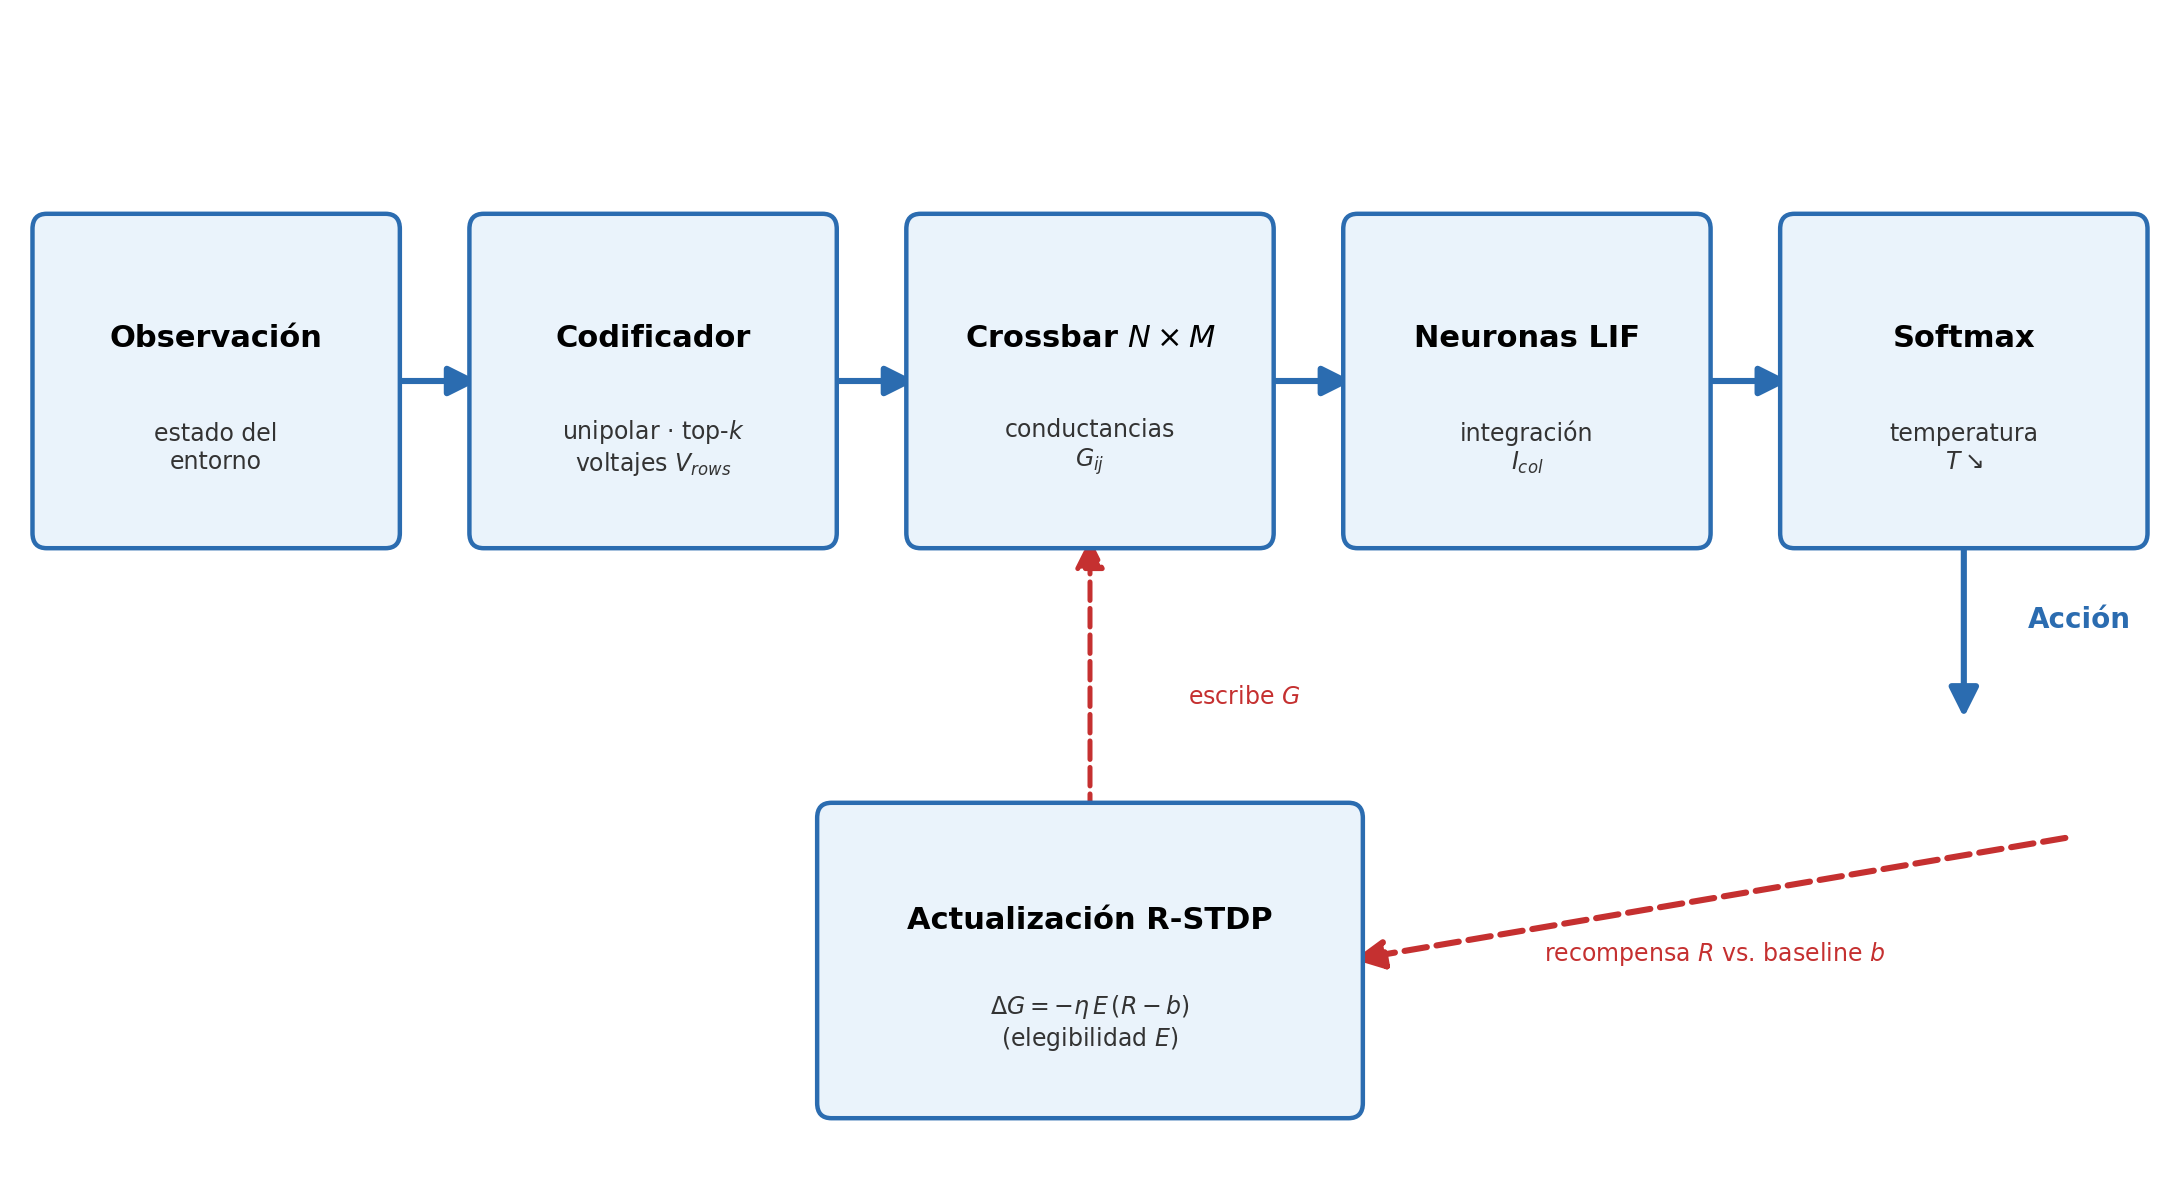
\includegraphics[width=\textwidth]{figuras/agente_arquitectura.png}
\caption{Arquitectura del agente neuromórfico. La observación 
se codifica en voltajes de fila, se propaga por el crossbar, se 
integra en neuronas LIF, y se decodifica en una acción. El 
aprendizaje se aplica al final del episodio.}
\label{fig:agente_arquitectura}
\end{figure}

\begin{figure}[H]
\centering
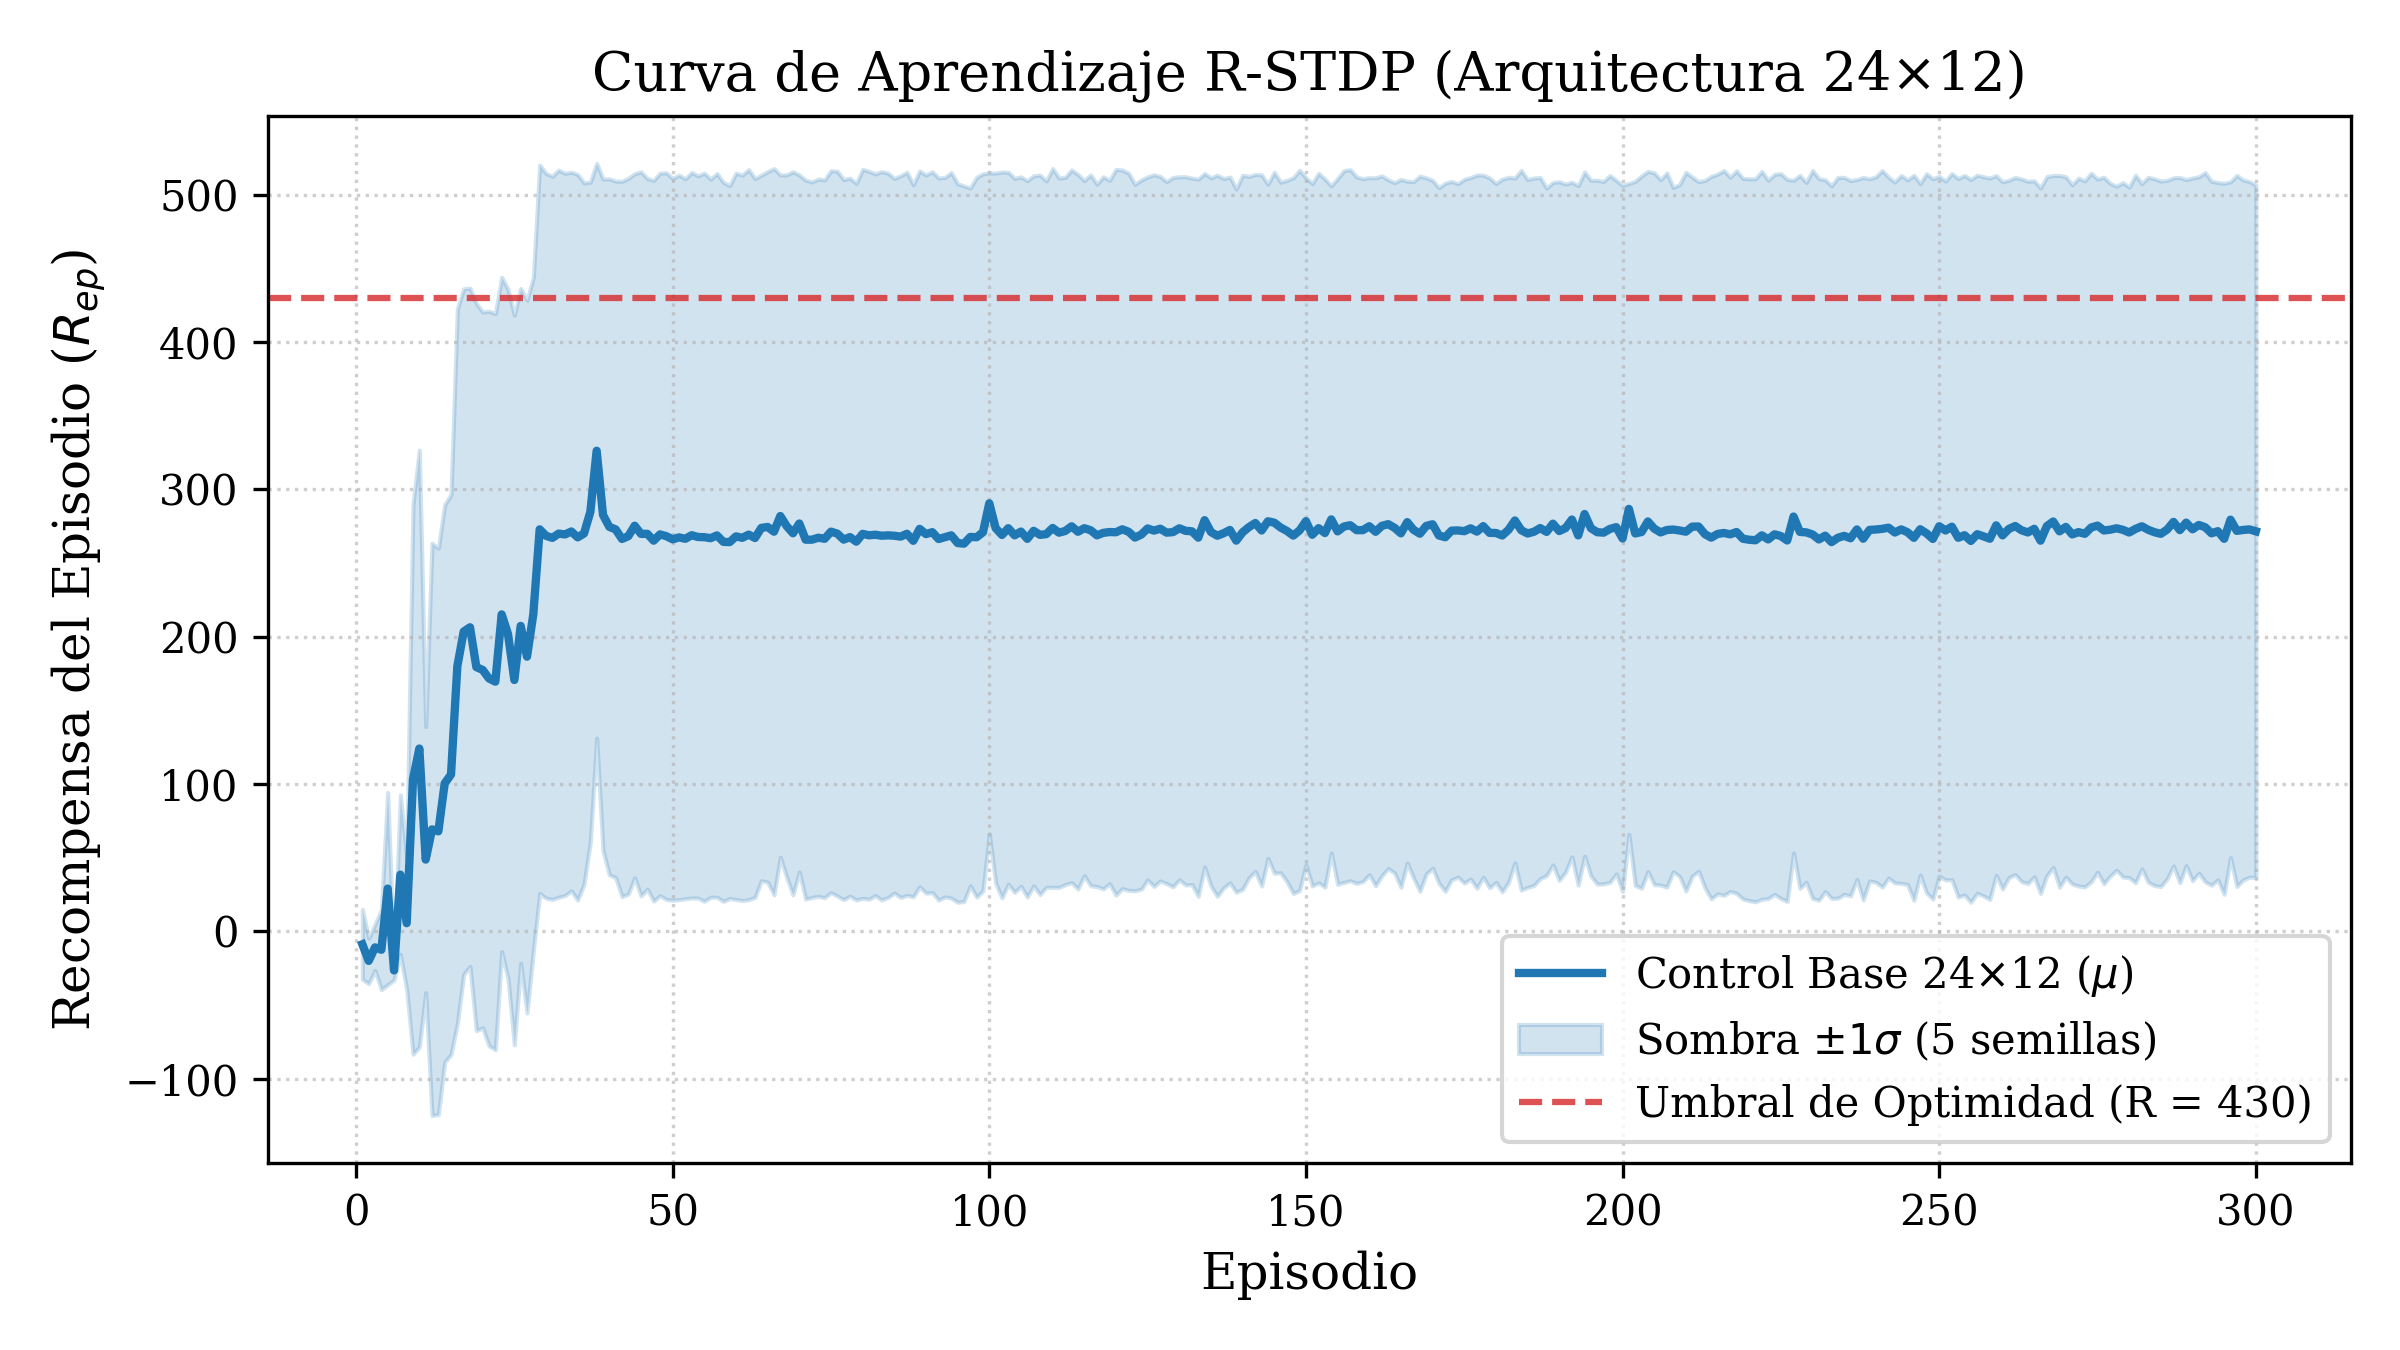
\includegraphics[width=0.85\textwidth]{figuras/cartpole_learning.png}
\caption{Curva de aprendizaje del agente en CartPole-v1. La 
media móvil sobre cinco semillas alcanza convergencia a la 
recompensa máxima en menos de 30 episodios.}
\label{fig:cartpole_learning}
\end{figure}
\subsection{Etapa 6 -- Extensión a percepción visual}

Para evaluar la generalidad del sustrato memristivo, el agente se 
extendió a un problema de clasificación de patrones visuales. El 
entorno define un conjunto de ocho patrones binarios de $8\times 8$ 
píxeles ---líneas, diagonales, cruces, marcos, la letra X y un 
cuadrado relleno--- y el agente debe reconocer la clase de la imagen 
presentada. Todos los experimentos se ejecutaron con el script 
\texttt{run\_vision.py} del repositorio, con 5000 episodios por 
semilla y tres semillas independientes.

\subsubsection{Codificación retinotópica}

La imagen se proyecta sobre las filas del crossbar mediante una 
codificación retinotópica unipolar: cada píxel activo se asigna a 
una fila del arreglo y se aplica un voltaje de lectura $V_{read}$ 
subumbral, mientras los píxeles inactivos permanecen a tierra. La 
asociación espacial píxel-fila preserva la topología de la imagen 
y mantiene todos los voltajes por debajo del umbral de escritura, 
garantizando una lectura no destructiva.

\subsubsection{Multiplicación analógica por el crossbar}

La operación central es el producto vector-matriz analógico 
$I = G \cdot V$: cada columna $j$ acumula la corriente pesada por 
las conductancias de sus 64 filas, obteniendo en un único ciclo de 
lectura una evidencia por cada una de las ocho clases. El arreglo 
de $64 \times 8$ elementos actúa entonces como un banco de 
clasificadores lineales cuyos pesos son las propias conductancias 
físicas del dispositivo, sin cómputo digital intermedio.

\subsubsection{Competencia blanda entre columnas}

Las corrientes de columna se normalizan y se transforman en una 
distribución de probabilidad mediante una función softmax. Este 
mecanismo equivale a una inhibición lateral de tipo 
winner-take-all en su forma suave: las clases compiten por la 
evidencia de corriente acumulada y el máximo de la distribución 
determina la clase predicha, permitiendo además el muestreo 
estocástico de decisiones durante el entrenamiento.

\subsubsection{Aprendizaje R-STDP supervisado}

El aprendizaje emplea la supervisión implícita del error de 
clasificación. Tras cada presentación se acumula una traza de 
elegibilidad $E$ ponderada por la diferencia entre la acción 
elegida y la distribución de la política, de modo que las 
conexiones que alimentaron a la clase seleccionada se refuerzan 
o deprimen según la señal de recompensa relativa $R - b$ contra 
una línea base móvil. La actualización usa la misma regla R-STDP 
del agente de control, confinando las conductancias al rango 
físico $[0,1]$ y limitando la norma del gradiente para preservar 
la estabilidad. Las tres semillas alcanzaron 100\% de acierto en 
los últimos 500 episodios.

La Figura~\ref{fig:vision_arquitectura} presenta el flujo completo 
de clasificación. La Figura~\ref{fig:vision_learning} muestra la 
curva de aprendizaje de la semilla 0, y la 
Figura~\ref{fig:vision_seeds} consolida la robustez de las tres 
semillas independientes.

\begin{figure}[H]
\centering
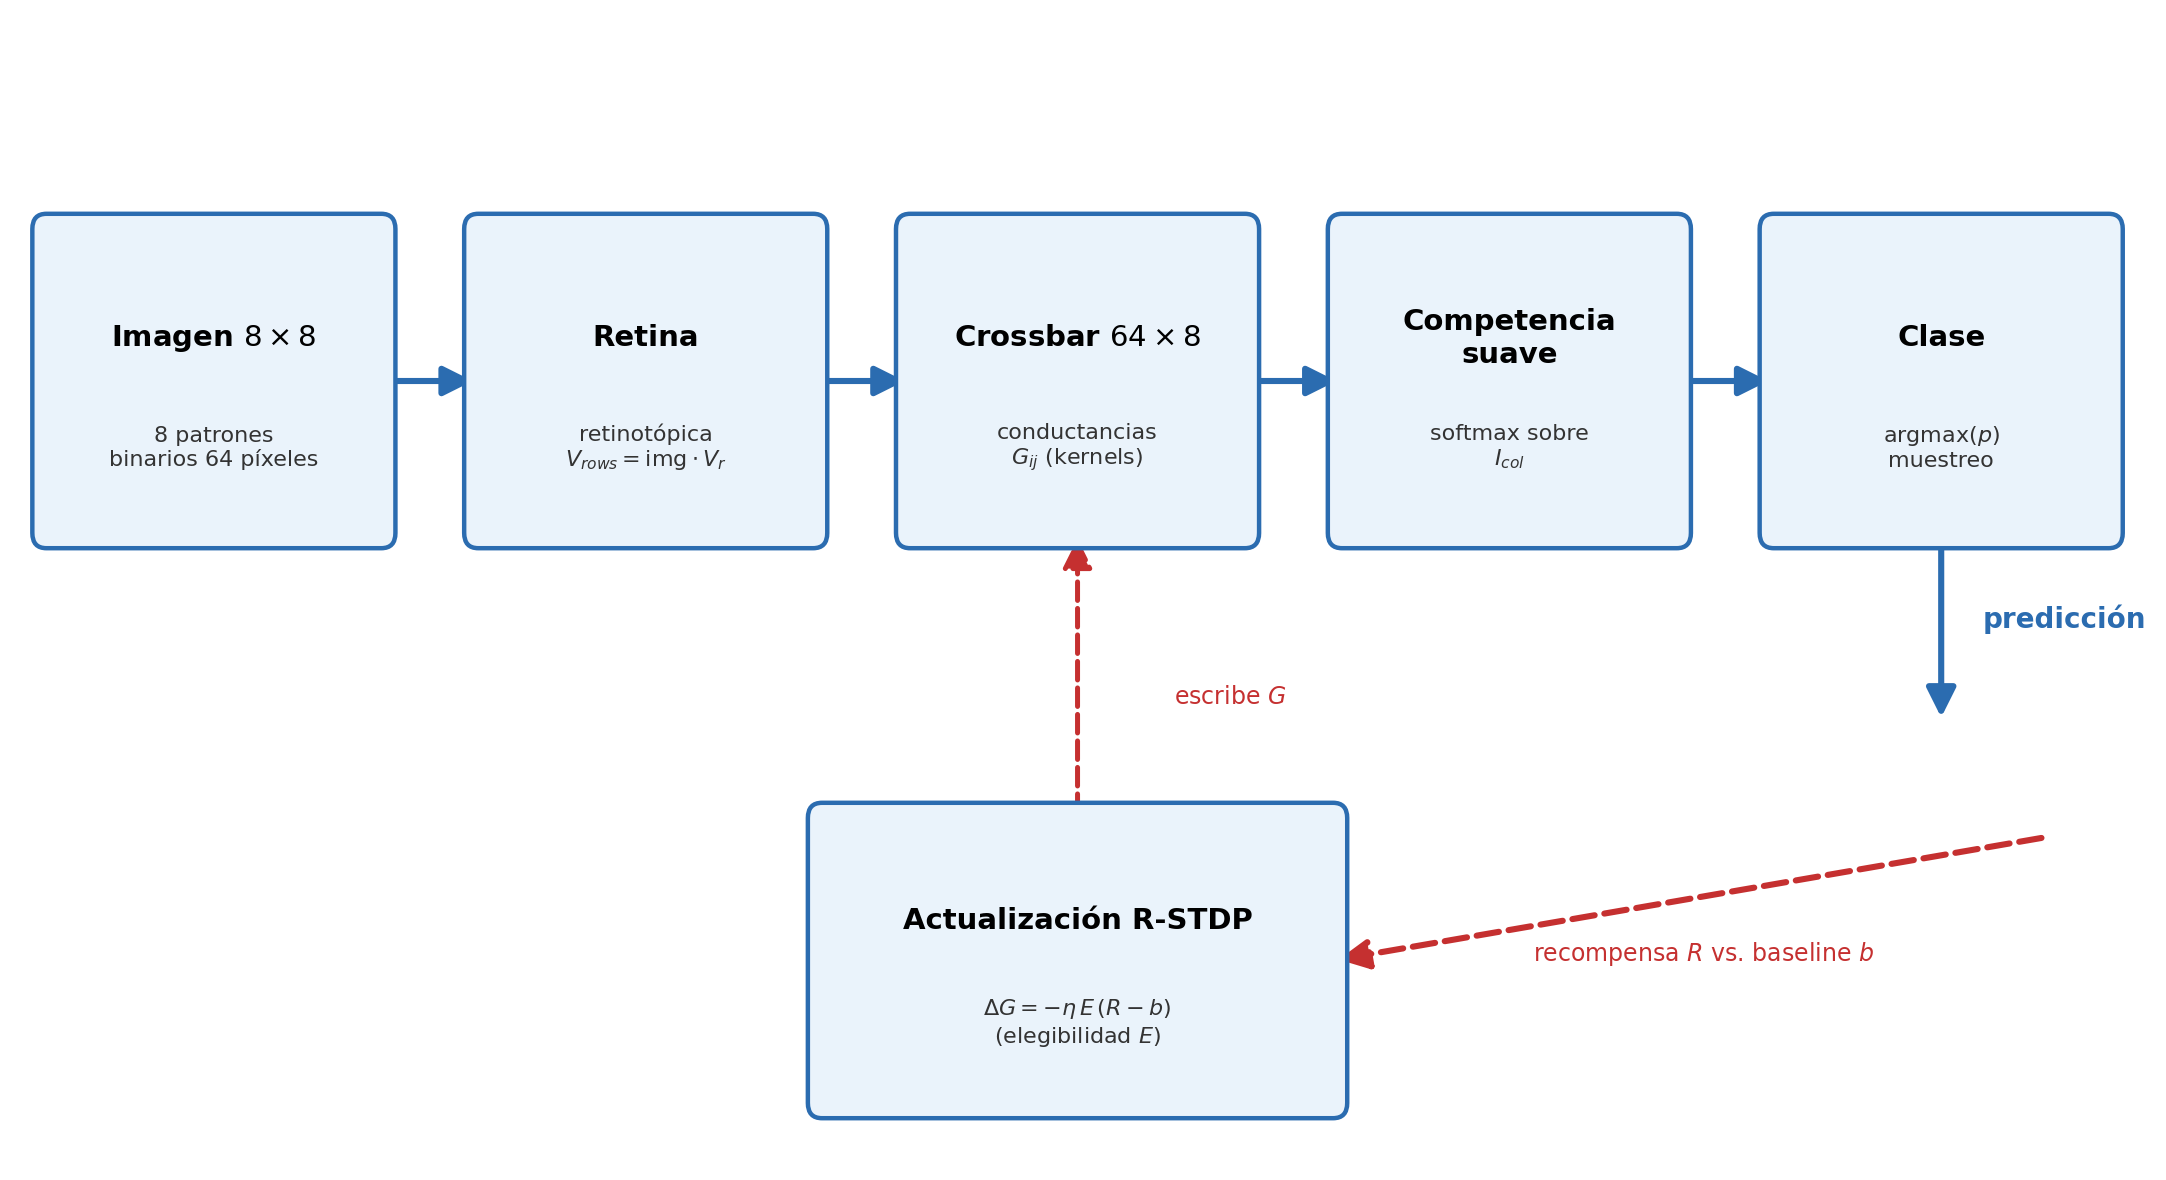
\includegraphics[width=\textwidth]{figuras/vision_arquitectura.png}
\caption{Arquitectura del clasificador neuromórfico. La imagen se 
codifica en voltajes de fila, se propaga por el crossbar $64\times 
8$, y la corriente de cada columna se normaliza en una 
distribución de probabilidad sobre las clases.}
\label{fig:vision_arquitectura}
\end{figure}

\begin{figure}[H]
\centering
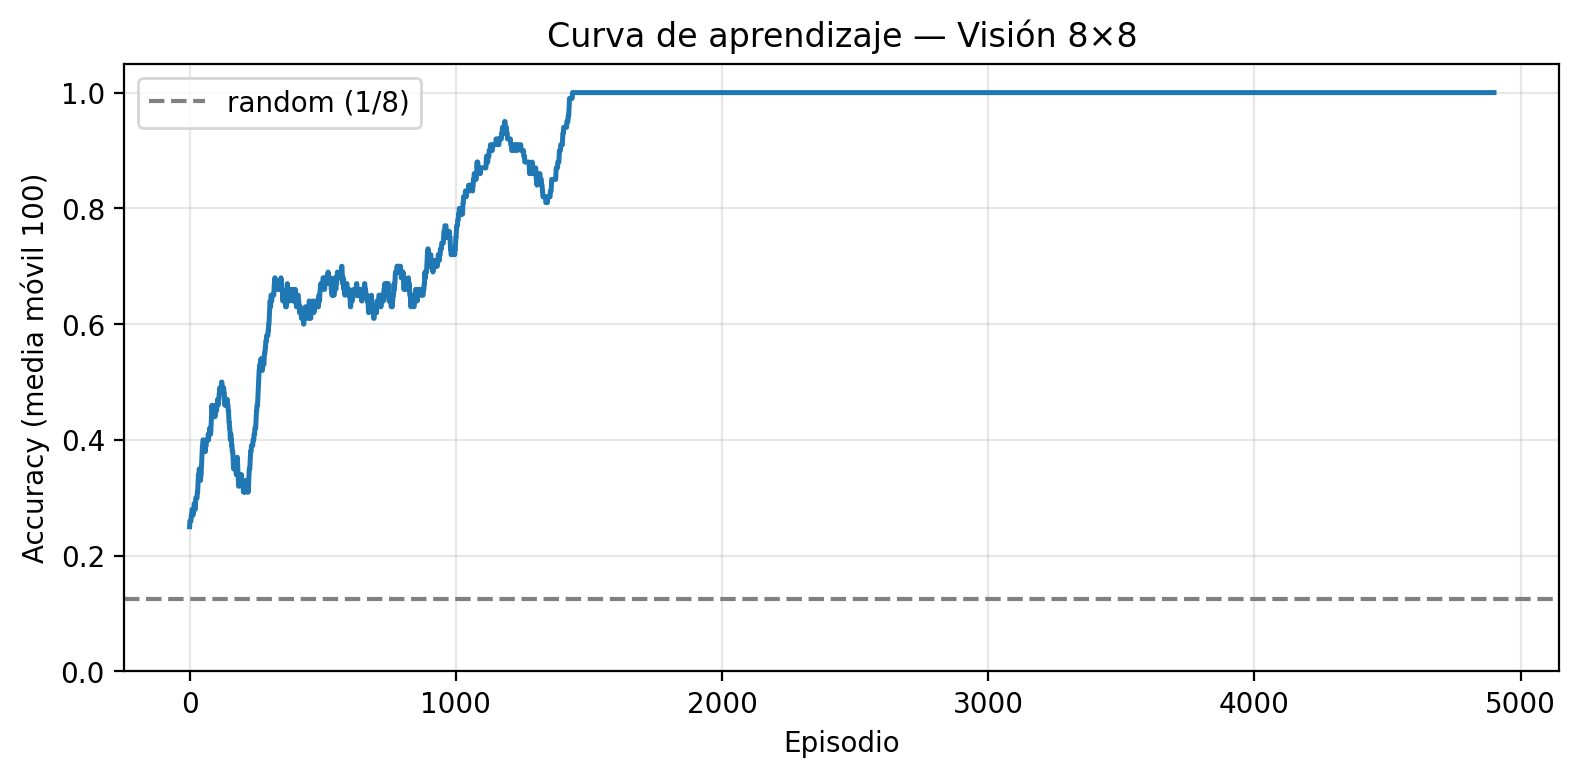
\includegraphics[width=0.8\textwidth]{figuras/vision_learning.png}
\caption{Curva de aprendizaje del clasificador sobre los ocho 
patrones, semilla 0. Media móvil de 100 episodios; la línea 
discontinua marca el nivel aleatorio $1/8$.}
\label{fig:vision_learning}
\end{figure}

\begin{figure}[H]
\centering
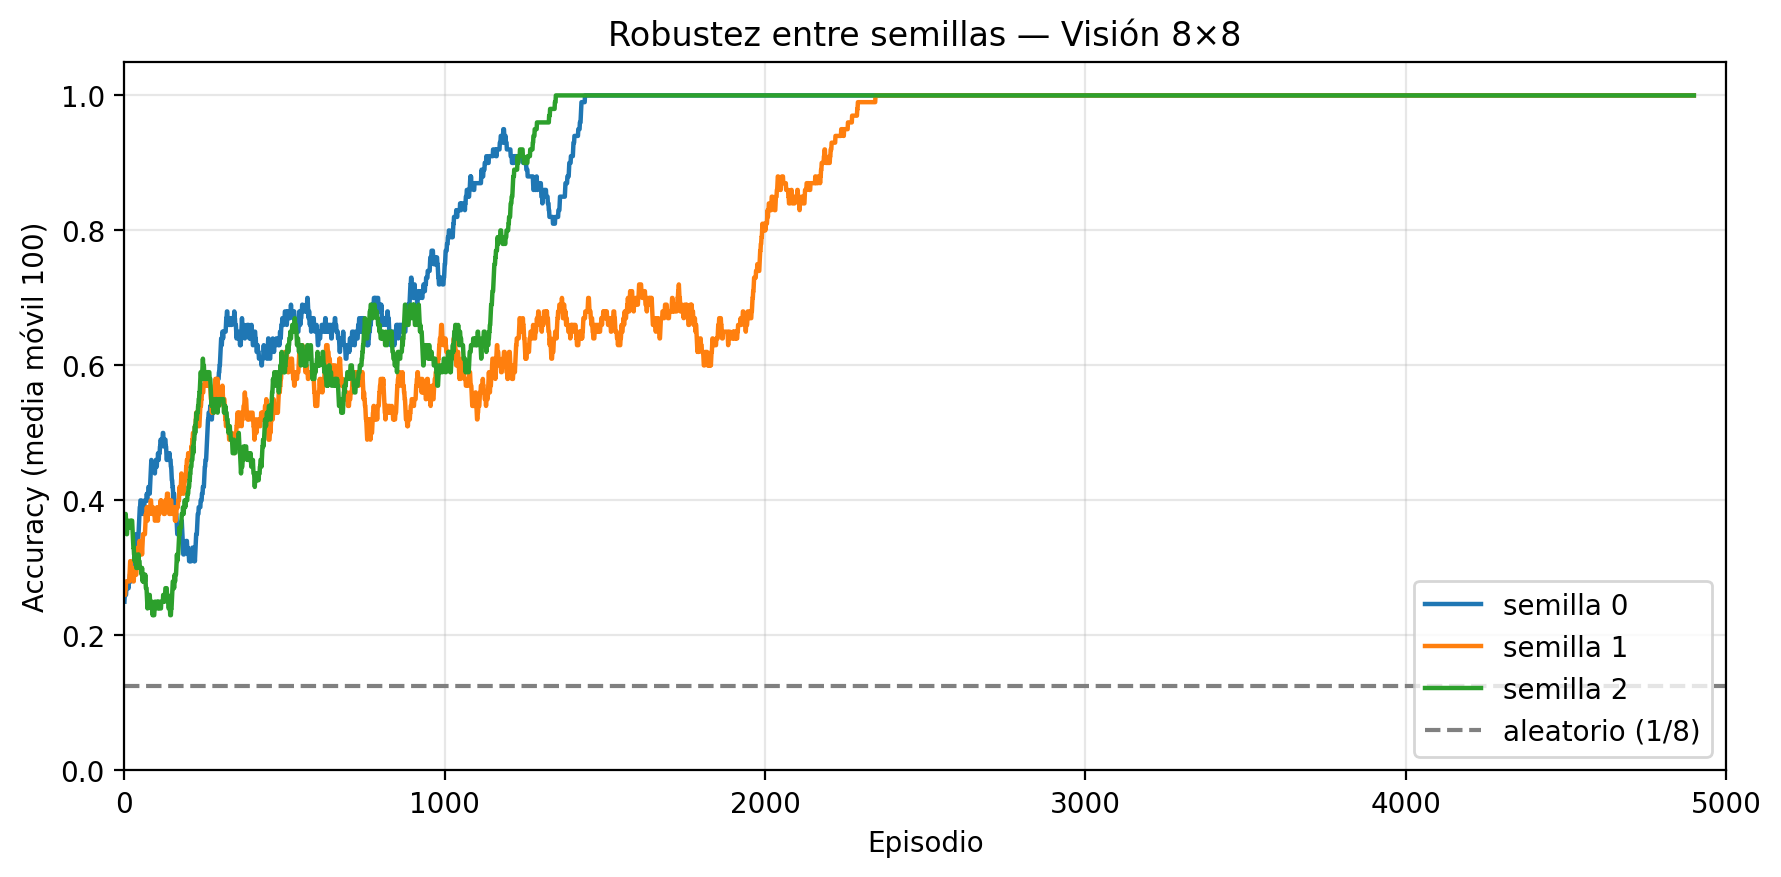
\includegraphics[width=\textwidth]{figuras/vision_seeds.png}
\caption{Robustez entre semillas: las tres corridas independientes 
(5000 episodios cada una) convergen a 100\% de acierto sobre los 
ocho patrones.}
\label{fig:vision_seeds}
\end{figure}
\subsection{Etapa 7 -- Navegación autónoma con obstáculos}

Para demostrar la versatilidad del sustrato memristivo en un 
segundo dominio de control, el mismo agente R-STDP se aplicó a un 
problema de navegación espacial. Se definió un entorno de tipo 
gridworld de $10 \times 10$ celdas con quince posiciones de 
obstáculo fijas (15\% del total), un punto de inicio en la esquina 
inferior izquierda y una meta en la esquina superior derecha. La 
disposición de obstáculos es determinística por semilla y se 
verifica que preserve al menos un camino válido entre ambos 
extremos. El agente dispone de cuatro acciones (arriba, abajo, 
izquierda y derecha), y la meta debe alcanzarse en un máximo de 
100 pasos.

\subsubsection{Sensor y codificación}

La observación combina un parche retinotópico de $3\times 3$ 
alrededor del agente ---nueve valores que distinguen obstáculo, 
celda libre y meta--- con la posición normalizada (dos componentes), 
totalizando once entradas. El vector se proyecta sobre las dieciséis 
filas del crossbar mediante el mismo codificador unipolar con 
selección top-$k$ ya descrito, y la acción se decodifica desde las 
cuatro columnas a través de las neuronas LIF con inhibición lateral.

\subsubsection{Recompensa}

La recompensa es escasa pero con la señal de meta amplificada: 
$+10$ al llegar a la meta, $-0.01$ por paso y $-0.1$ por colisión. 
La amplificación del componente de meta se introdujo para que la 
señal episódica $R_{ep}-b$ quede dominada por el evento de éxito 
frente a la magnitud acumulada de pasos y colisiones, condición 
necesaria para que REINFORCE episódico pueda asignar crédito a la 
trayectoria completa.

\subsubsection{Resultados}

La tasa de éxito de una política aleatoria sobre este entorno es 
del 4.2\%. Tras 800 episodios por semilla, las tres corridas 
independientes superan ampliamente ese nivel: la mejor semilla 
alcanza un 99\% de acierto en los últimos 100 episodios y un 82\% 
en los últimos 200, con un promedio del 67\% entre las tres. El 
roll-out determinístico de la política aprendida con la mejor 
semilla llega a la meta en 19 pasos. Además, a diferencia de lo 
observado en la clasificación visual, la matriz de pesos del 
crossbar sí se especializa de forma marcada: la desviación 
estándar de $X$ crece a 0.29--0.34 mientras su media asciende de 
0.10 a 0.34, evidenciando que la navegación exige un reordenamiento 
estructural de las conductancias.

La Figura~\ref{fig:obstacle_mapa} presenta el entorno de 
navegación. La Figura~\ref{fig:obstacle_trayectoria} compara la 
trayectoria aleatoria inicial con la política aprendida, la 
Figura~\ref{fig:obstacle_learning} consolida las curvas de las tres 
semillas, y la Figura~\ref{fig:obstacle_arquitectura} resume la 
arquitectura del sistema.

\begin{figure}[H]
\centering
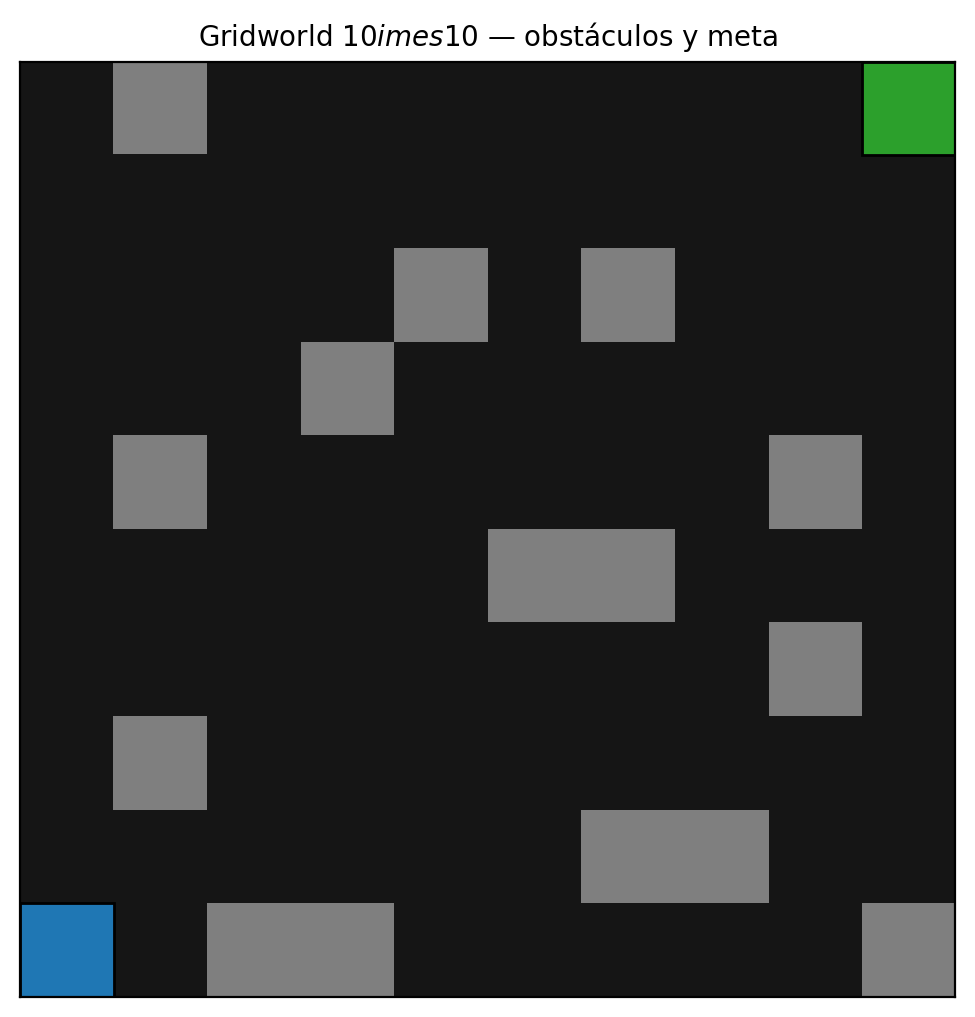
\includegraphics[width=0.6\textwidth]{figuras/obstacle_mapa.png}
\caption{Entorno de navegación: gridworld $10\times10$ con quince 
celdas de obstáculo (gris), punto de inicio (azul) y meta (verde). 
La disposición es determinística por semilla y garantiza un camino 
válido.}
\label{fig:obstacle_mapa}
\end{figure}

\begin{figure}[H]
\centering
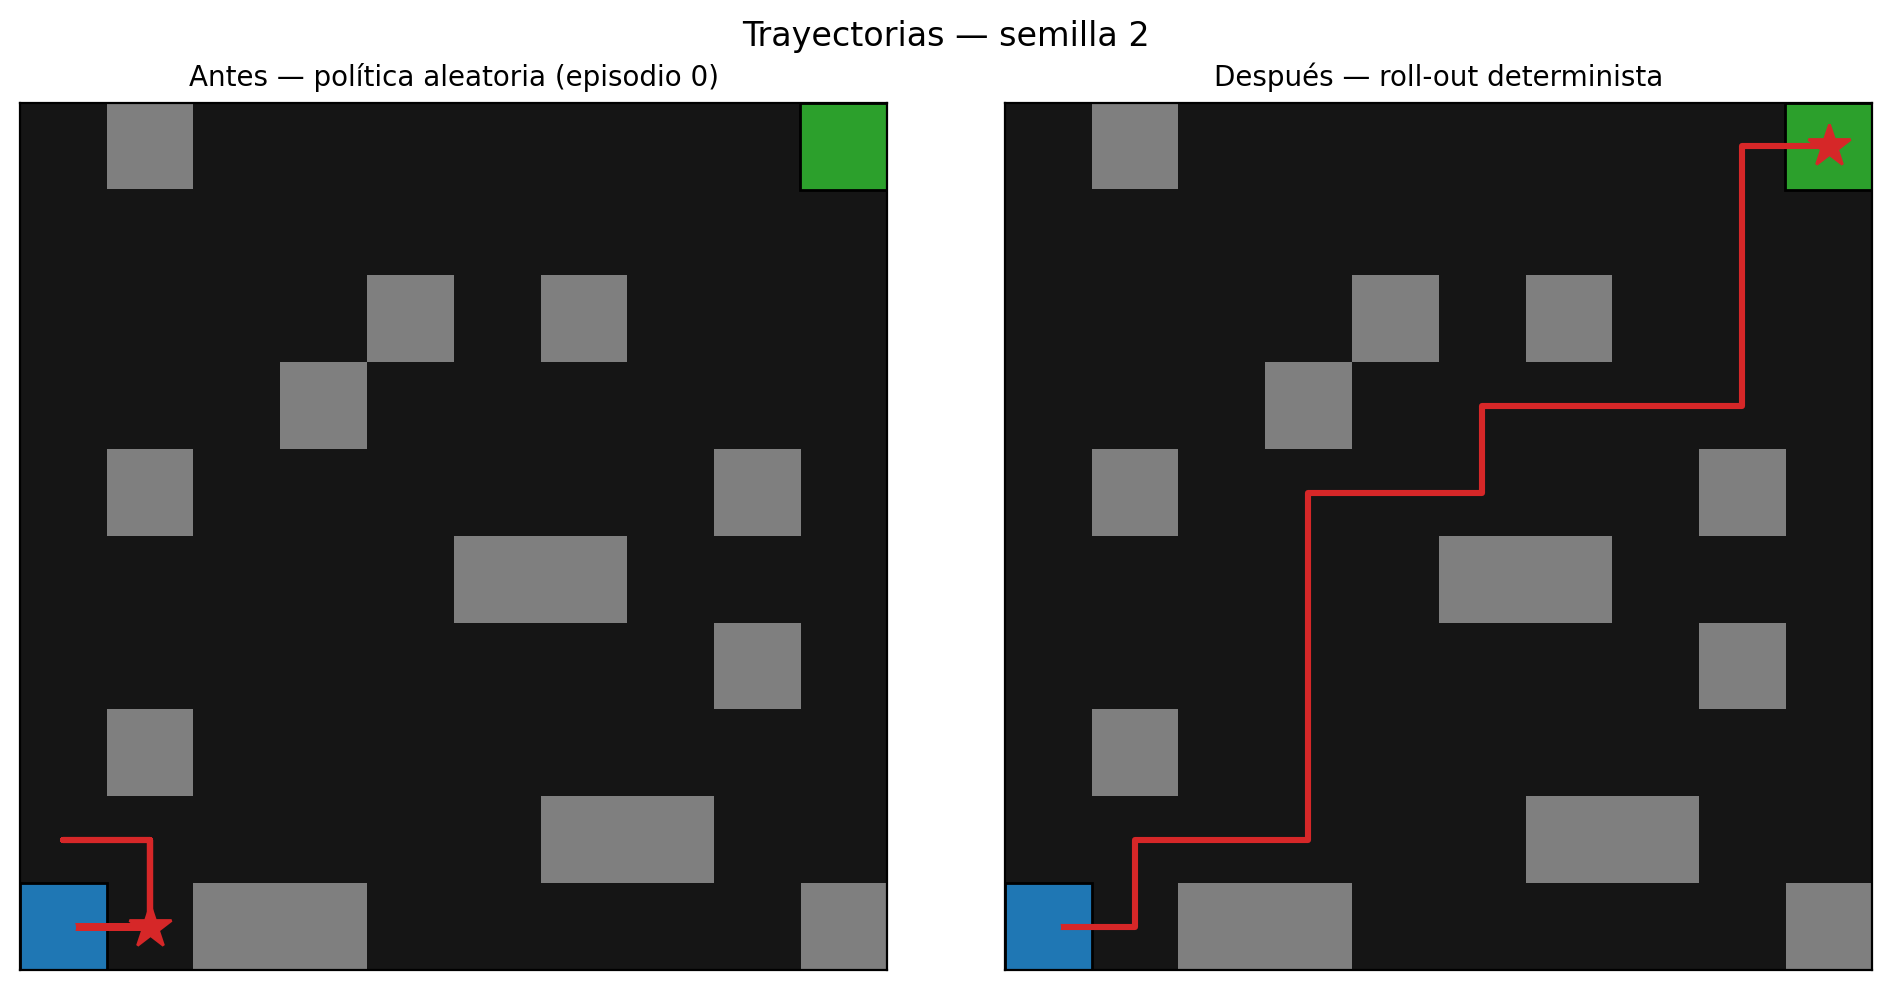
\includegraphics[width=\textwidth]{figuras/obstacle_trayectoria.png}
\caption{Trayectorias sobre el entorno de la semilla 2. Izquierda: 
episodio 0 con política aleatoria. Derecha: roll-out determinístico 
de la política aprendida, que alcanza la meta en 19 pasos.}
\label{fig:obstacle_trayectoria}
\end{figure}

\begin{figure}[H]
\centering
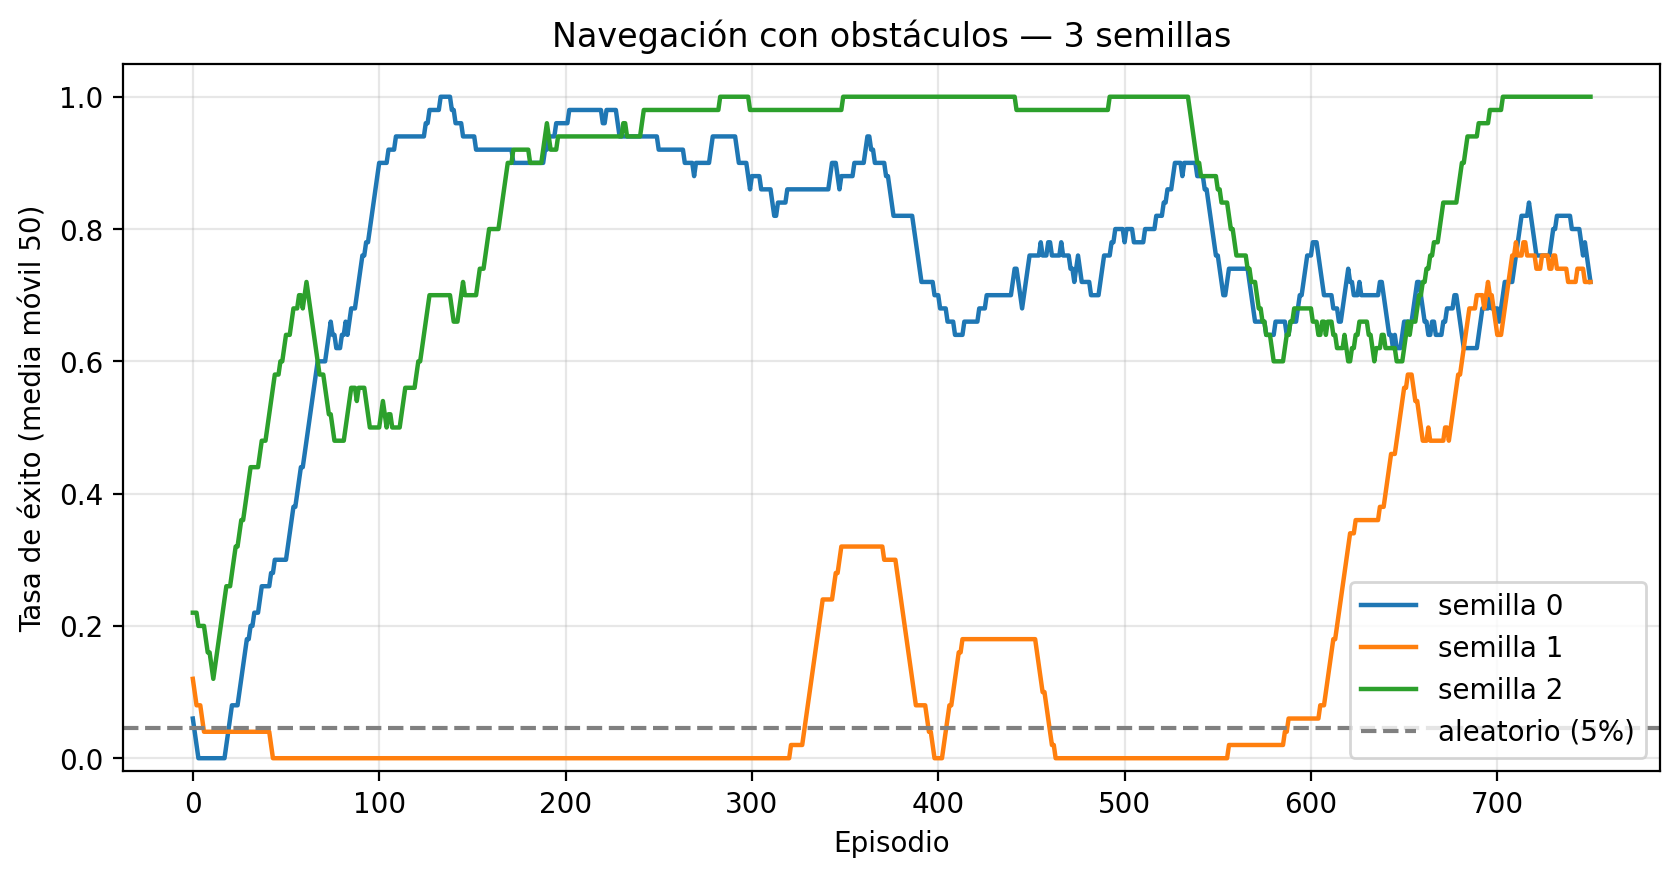
\includegraphics[width=0.85\textwidth]{figuras/obstacle_learning.png}
\caption{Tasa de éxito de la navegación (media móvil de 50 
episodios) para las tres semillas. La línea discontinua marca el 
nivel aleatorio (4.2\%) y la mejor semilla converge a 99\%.}
\label{fig:obstacle_learning}
\end{figure}

\begin{figure}[H]
\centering
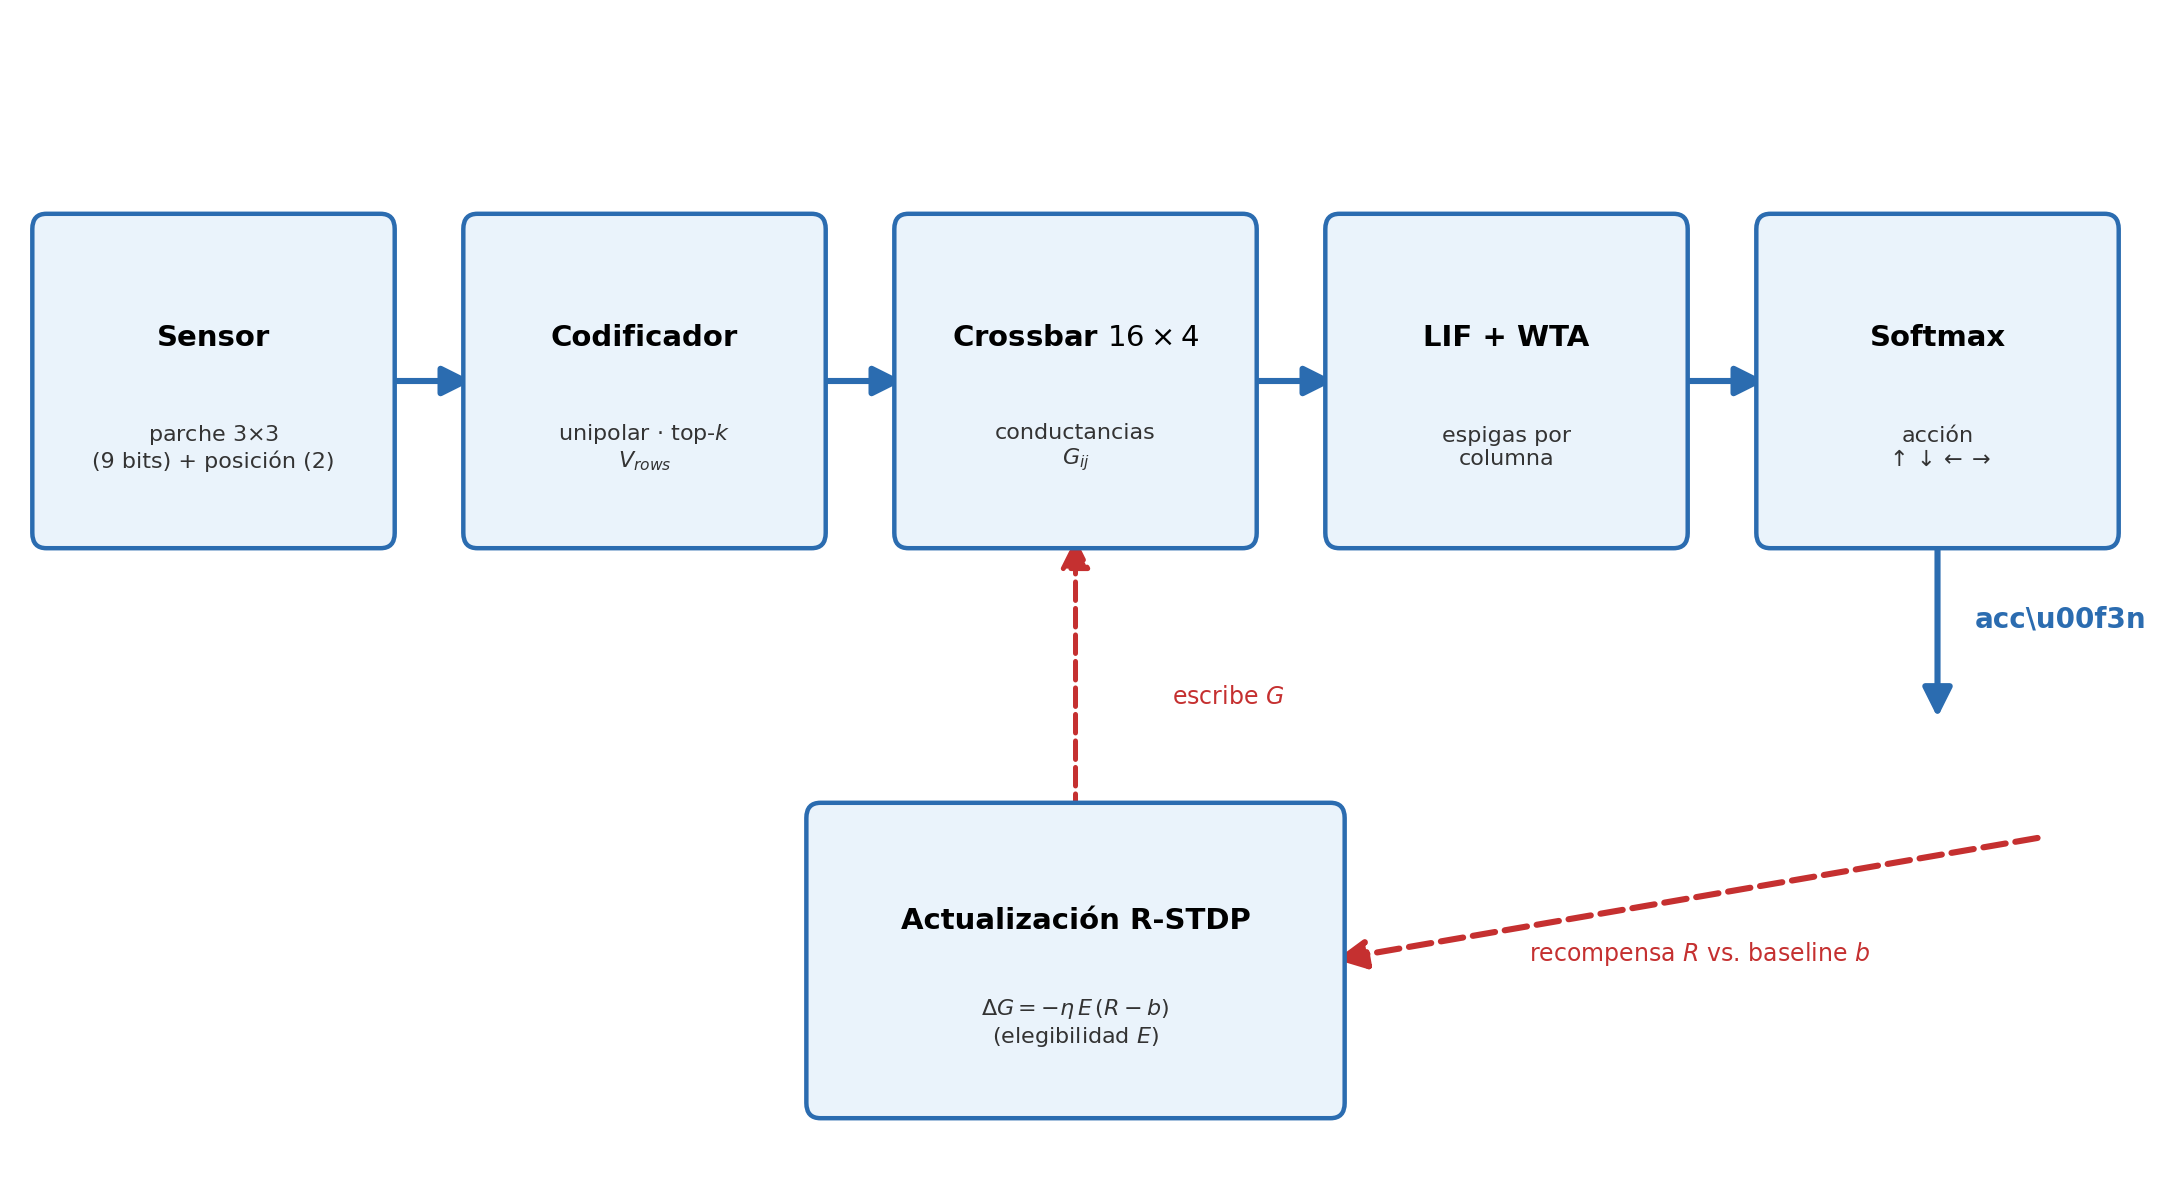
\includegraphics[width=\textwidth]{figuras/obstacle_arquitectura.png}
\caption{Arquitectura del agente de navegación. El mismo 
crossbar R-STDP de las etapas anteriores, con $N=16$ filas y 
$M=4$ columnas, procesa el parche sensorial $3\times 3$ y la 
posición para producir la acción.}
\label{fig:obstacle_arquitectura}
\end{figure}
% =====================================================
\section{Resultados y discusión}
% =====================================================

% (vacío por ahora)

% =====================================================
\section{Análisis de costos}
% =====================================================

% (vacío por ahora)
